% Template for PLoS
% Version 3.4 January 2017
\documentclass[10pt,letterpaper]{article}
\usepackage[top=0.85in,left=2.75in,footskip=0.75in]{geometry}

% amsmath and amssymb packages, useful for mathematical formulas and symbols
\usepackage{amsmath,amssymb}

% Use adjustwidth environment to exceed column width (see example table in text)
\usepackage{changepage}

% Use Unicode characters when possible
\usepackage[utf8x]{inputenc}

% textcomp package and marvosym package for additional characters
\usepackage{textcomp,marvosym}

% cite package, to clean up citations in the main text. Do not remove.
% \usepackage{cite}

% Use nameref to cite supporting information files (see Supporting Information section for more info)
\usepackage{nameref,hyperref}

% line numbers
\usepackage[right]{lineno}

% ligatures disabled
\usepackage{microtype}
\DisableLigatures[f]{encoding = *, family = * }

% color can be used to apply background shading to table cells only
\usepackage[table]{xcolor}

% array package and thick rules for tables
\usepackage{array}

% create "+" rule type for thick vertical lines
\newcolumntype{+}{!{\vrule width 2pt}}

% create \thickcline for thick horizontal lines of variable length
\newlength\savedwidth
\newcommand\thickcline[1]{%
  \noalign{\global\savedwidth\arrayrulewidth\global\arrayrulewidth 2pt}%
  \cline{#1}%
  \noalign{\vskip\arrayrulewidth}%
  \noalign{\global\arrayrulewidth\savedwidth}%
}

% \thickhline command for thick horizontal lines that span the table
\newcommand\thickhline{\noalign{\global\savedwidth\arrayrulewidth\global\arrayrulewidth 2pt}%
\hline
\noalign{\global\arrayrulewidth\savedwidth}}


% Remove comment for double spacing
%\usepackage{setspace}
%\doublespacing

% Text layout
\raggedright
\setlength{\parindent}{0.5cm}
\textwidth 5.25in
\textheight 8.75in

% Bold the 'Figure #' in the caption and separate it from the title/caption with a period
% Captions will be left justified
\usepackage[aboveskip=1pt,labelfont=bf,labelsep=period,justification=raggedright,singlelinecheck=off]{caption}
\renewcommand{\figurename}{Fig}

% Use the PLoS provided BiBTeX style
% \bibliographystyle{plos2015}

% Remove brackets from numbering in List of References
\makeatletter
\renewcommand{\@biblabel}[1]{\quad#1.}
\makeatother

% Leave date blank
\date{}

% Header and Footer with logo
\usepackage{lastpage,fancyhdr,graphicx}
\usepackage{epstopdf}
\pagestyle{myheadings}
\pagestyle{fancy}
\fancyhf{}
\setlength{\headheight}{27.023pt}
\lhead{
\includegraphics[width=2.0in]{PLOS-submission.eps}}
\rfoot{\thepage/\pageref{LastPage}}
\renewcommand{\footrule}{\hrule height 2pt \vspace{2mm}}
\fancyheadoffset[L]{2.25in}
\fancyfootoffset[L]{2.25in}
\lfoot{\sf PLOS}

%% Include all macros below
\newcommand{\lorem}{{\bf LOREM}}
\newcommand{\ipsum}{{\bf IPSUM}}


\usepackage{booktabs}



\usepackage{forarray}
\usepackage{xstring}
\newcommand{\getIndex}[2]{
  \ForEach{,}{\IfEq{#1}{\thislevelitem}{\number\thislevelcount\ExitForEach}{}}{#2}
}

\setcounter{secnumdepth}{0}

\newcommand{\getAff}[1]{
  \getIndex{#1}{McMaster University,The Hong Kong Polytechnic University,University of Toronto}
}

\providecommand{\tightlist}{%
  \setlength{\itemsep}{0pt}\setlength{\parskip}{0pt}}

\begin{document}
\vspace*{0.2in}

% Title must be 250 characters or less.
\begin{flushleft}
{\Large
\textbf\newline{Demand and Supply Inflation in Floating Catchment Area (FCA) Methods
(TEST)} % Please use "sentence case" for title and headings (capitalize only the first word in a title (or heading), the first word in a subtitle (or subheading), and any proper nouns).
}
\newline
\\
Antonio Paez\textsuperscript{\getAff{McMaster University}}\textsuperscript{*},
Christopher D. Higgins\textsuperscript{\getAff{The Hong Kong Polytechnic University}},
Salvatore F. Vivona\textsuperscript{\getAff{University of Toronto}}\\
\bigskip
\textbf{\getAff{McMaster University}}School of Geography and Earth Sciences, McMaster University, 1280 Main
St W, Hamilton, ON L8S 4K1 Canada\\
\textbf{\getAff{The Hong Kong Polytechnic University}}Department of Land Surveying and Geo-Informatics \& Department of
Building and Real Estate, 11 Yuk Choi Rd, Hung Hom, Hong Kong\\
\textbf{\getAff{University of Toronto}}Department of Computer Science, University of Toronto, 214 College
Street, Toronto, ON, M5T 3A1\\
\bigskip
* Corresponding author: paezha@mcmaster.ca\\
\end{flushleft}
% Please keep the abstract below 300 words
\section*{Abstract}
Floating Catchment Area (FCA) methods have become a very popular tool to
investigate accessibility to public facilities, in particular health
care services. FCA approaches are attractive because, unlike other
accessibility measures, they take into account the potential for
congestion of facilities. This is done by considering the population
within the catchment area of a facility to calculate a variable that
measures level of service, and then aggregating the level of service by
population centers subject to catchment area constraints. In this paper
we discuss what seems to be a hitherto overlooked effect of FCA
approaches, an artifact that we term demand and supply \emph{inflation}.
We show 1) how these artifacts are present in 2FCSA, E2FSCA, and 3SFCA;
and 2) how they lead to misleading estimates of accessibility, with
possible deleterious consequences for decision making. Next, we propose
a simple and intuitive approach to adjust the impedance weights used in
the calculation of FCAs that rectifies the inflation effect. The result
is a more intiuitive measure of accessibility that 1) provides a local
version of the provider-to-population ratio; and 2) preserves the level
of demand and the level of supply in a system. We illustrate the
relevant issues with some simple examples, and then empirically by means
of a case study of accessibility to family physicians in the Hamilton
Census Metropolitan Area (CMA), in Ontario, Canada. Results indicate
that demand and supply inflation/deflation poses a serious problem for
the interpretation of accessibility analysis using existing FCA methods,
and that these issues that are eliminated through the use of the
proposed adjustments.

% Please keep the Author Summary between 150 and 200 words
% Use first person. PLOS ONE authors please skip this step.
% Author Summary not valid for PLOS ONE submissions.

\linenumbers

% Use "Eq" instead of "Equation" for equation citations.
\section{Introduction}\label{introduction}

Evaluating accessibility to healthcare services is an important issue in
health geography and health policy, with hundreds of research papers
published on the topic since the 2000s {[}1{]}. However, the concept of
accessibility is multi-dimensional, which often presents challenges to
its operationalization in empirical research. According to Joseph and
Bantock {[}2{]}, accessibility can be defined by both aspatial and
spatial dimensions. The first dimension considers factors such as the
availability of healthcare services (or the supply of services), their
potential or revealed use by the public (demand). Other aspatial factors
include the characteristics of the supply, such as the cost of utilizing
the service, and the characteristics of the individual, such as their
income, social class, ethnicity, and mobility profile. The spatial
dimension considers the geographic distribution of available healthcare
services and the costs or friction involved in travelling to them. By
taking these dimensions into account, estimates of accessibility can
identify areas with high or low access to healthcare services and
provide critical information related to social and spatial inequalities
and guidance for health policy and resource allocation.

At a high level, provider-to-population ratios offer some indication of
the level of service within a community. However, these measures lack a
true spatial dimension. In contrast, gravity measures offer a more
sophisticated approach to measuring spatial accessibility to healthcare
{[}2{]}. Nevertheless, these methods have been criticized for the
difficulty involved in specifying a suitable distance decay function
{[}3{]}. From this, one of the most popular approaches to estimating
healthcare accessibility in the previous literature is the Two-Step
Floating Catchment Area (2SFCA) method proposed by Luo and Wang
{[}4,5{]}, which is based on a simplified gravity model with a binary
distance function. Numerous applications are found in the international
literature, including work from Germany {[}6{]}, South Korea {[}7{]},
Japan {[}8{]}, China {[}9{]}, Australia {[}10{]}, and Canada {[}11{]}.

Within the 2SFCA framework, accessibility to healthcare is estimated
across two stages: in the first, the PPR at a given healthcare provider
is determined based on the number of physicians and the estimated demand
from the surrounding population within some catchment area. In the
second stage, the level of service for different healthcare providers is
summarized for the population. By simplifying gravity measures and
operationalizing healthcare accessibility in terms of
population-to-provider ratios, the properties of the 2SFCA method make
it both intuitive and appealing for health policy.

Still, several improvements have been made to the 2SFCA method since it
was proposed that seek to address the method's most significant
perceived shortcomings. The result is a family of Floating Catchment
Areas (FCA) methods that include more realistic conceptualizations of
distance by specifying variable catchment area sizes {[}10{]} and/or the
incorporation of stepped {[}12{]}, continuous {[}13{]}, and adaptive
{[}14{]} distance-decay functions. Other authors have added multi-modal
transportation {[}15{]}, age-adjusted healthcare demand profiles
{[}16{]}, and ways to counteract the modifiable areal unit problem
{[}17{]}.

A second major focus area has been the addition of competition for
available opportunities or the allocation of services to regions. As we
discuss further in the next section, the original 2SFCA approach has
been criticized for over-estimating demand {[}18{]}. By summarizing the
population within the catchment area of healthcare facilities, the
original 2SFCA framework often produces double-counting that tends to
inflate estimates of the level of demand at supply points in the
healthcare system, which in turn deflates the level of service for
populations within the study area. Proposed solutions to this problem
include the addition of selection weights based on a travel impedance
function in what Wan et al. {[}18{]} refer to as the Three-Step Floating
Catchment Area (3SFCA) method and a modified 3SFCA that uses a Huff
model to probabalisticly estimate these selection weights {[}19{]} based
on impedance and the supply of physicians at a given facility. On the
supply side (the allocation of the service to populations), Delamater
{[}20{]} proposes a modification to the 2SFCA method to address what he
terms a ``suboptimal'' spatial configuration of services.

However, although the issue of demand overestimation (or inflation) and
the alloation of services has been correctly identified in the
literature, there are not to our knowledge any existing methods that
adequately solve these perceived shortcomings. As we will show, previous
approaches inflate or deflate demand and supply to varying degrees.
Crucially, this results in potentially misleading estimations of
healthcare accessibility. As a consequence, potentially erroneous
recommendations for health policy could result, including the imprecise
identification of spatial inequalities.

In response, this research proposes a simple and intuitive approach to
adjusting the impedance weights used in the estimation of FCA methods.
By incorporating methods drawn from the field of spatial econometrics,
we preserve levels of demand and supply in the system and eliminate the
inflation and deflation of these parameters in previous FCA
approaches.To illustrate the benefits of this approach, we conduct a
case study of access to family physicians in Hamilton, Canada. Our
results indicate that the proposed adjustments produce more intuitive
measures of accessibility to healthcare measured in terms of local
provider-to-population ratios. Moreover, these outputs can be used to
provide estimates of access disparity across a region that are both
easily understood and robust to demand and supply inflation.

\section{Demand Inflation/Accessibility Deflation in FCA
Methods}\label{demand-inflationaccessibility-deflation-in-fca-methods}

\subsection{Floating Catchment Area
Methods}\label{floating-catchment-area-methods}

To motivate the discussion to follow we begin by quickly reviewing some
popular FCA methods. In general terms, FCA approaches are implemented in
two steps (2SFCA). In the first step, \emph{catchment areas} are defined
for facilities (e.g., clinics, parks, libraries, etc.) by means of an
impedance function. The population within a catchment area is allocated
to the corresponding facility or service point. This creates a demand or
congestion effect. More formally, the level of demand \(D_{j}\) is
calculated using a combination of the population at \(i\) and an
impedance function \(W\) that depends on \(d_{ij}\), an indicator of the
cost of travel between \(i\) and \(j\) (e.g., distance, travel time,
out-of-pocket expenses, or generalized cost): \[
D_j = \sum_i{D_{ij}} = \sum_i{P_iW(d_{ij})}
\]

Next, the level of supply at the facility is then divided by the demand
to obtain a measure of level of service (e.g., beds/person, sq.m of park
space/person, library floor space/person). Here, the level of service at
location \(j\) is defined as follows (decomposed in various ways): \[
L_j = \frac{S_j}{D_j} = \frac{S_j}{\sum_iD_{ij}} = \sum_i\frac{S_j}{D_{ij}}=\sum_iL_{ij}
\] where \(S_i\) is the supply of the service offered at location \(j\)
(say, number of beds/doctors in a clinic), whereas \(D_j\) is the level
of demand on that service location. It is clear that the congestion
effect results from the level of demand, which in turn depends on the
number of potential users from different origins \(i\) that converge at
service point \(j\): at a fixed level of supply, greater demand results
in lower levels of service. The different decompositions of \(L_j\) help
to understand how different population centers influence the level of
demand at \(j\).

In the second step, the catchment areas are ``floated'' to the
population centers. Accessibility at location \(i\), in turn, is defined
as the weighted sum (via the impedance function) of the level of service
at every location \(j\) that includes \(i\) within its catchment area:
\[
A_i = \sum_j{L_jW(d_{ij})}
\] \#\# FCA Impedance Function

The impedance function incorporated into both steps of the 2SFCA
technique implements the geographical concept of distance-decay, which
reflects a commonly observed cost-minimization behavior, namely that
people in general prefer to spend less time than more travelling to
destinations. In effect, the impedance function defines the
\emph{catchment areas} for the points of service and population centers
alike.

In early implementations of the 2SFCA approach {[}4{]}, a binary
impedance function was used: \[
D_j = \sum_iD_{ij} = \sum_iP_iW(d_{ij}|d_0)
\]

with: \[
W(d_{ij}\leq d_0) = \left\{
        \begin{array}{ll}
            1 & \quad d_{ij} \leq d_0 \\
            0 & \quad d_{ij} > d_0
        \end{array}
    \right.
\]

This formulation assumes equal potential for use within a catchment
area, and zero beyond. In other words, travellers are assumed to be
equally likely users of a service point within the catchment area,
irrespective of how proximate or distant they are from it.

A criticism of the binary impedance function is that it does not account
for the declining probability of using a facility as distance grows. As
a result of this criticism, other impedance functions have since been
proposed, including the stepwise formulation of the Enhanced 2-Step
Floating Catchment Area method {[}12{]}: \[
D_j = \sum_iD_{ij} = \sum_{i=1}^N\sum_{r=1}^R P_iW(d_{ij}|d_1, d_2, \dots, d_R)
\] where \(W(d_{ij}|d_1, d_2, \dots, d_R)\) takes different values
depending on the value of \(d_{ij}\) and cost threshold values \(d_r\),
as follows: \[
W(d_{ij}) = \left\{
        \begin{array}{ll}
            k_1 & \quad d_{ij} \leq d_1 \\
            k_2 & \quad d_1 < d_{ij} \leq d_2 \\
            \dotsb \\
            k_{R-1} & \quad d_{R-1} < d_{ij} \leq d_R \\
            0 & \quad d_{ij} > d_R
        \end{array}
    \right.
\]

Clearly, a stepwise function does not assume identical potential within
the extent of the catchment area (i.e., the space contained within
\(d_{ij} \leq d_R\)), and better reflects empirical observations of
travel behavior. More recent research has introduced smooth functions to
replace the stepwise approach. It is worthwhile noting that impedance
functions have long been studied in geographical analysis in general
{[}21{]}, and accessibility research in particular {[}22{]}, but it is
only relatively recently that alternative impedance functions have been
incorporated in FCA approaches. These include continuous functions
{[}13{]} and mixtures of continuous and step functions {[}3{]}.

\subsection{Demand and Supply Inflation in the
2SFCA}\label{demand-and-supply-inflation-in-the-2sfca}

An important point in the implementation of FCA methods {[}18{]}, is
that demand tends to be overestimated. This is a consequence of the way
in which \(Dj\) is calculated, which generally fails to preserve the
population. In other words, 2SFCA methods lack the pycnophilactic
property discussed by Tobler {[}23{]}. In practical terms, this implies
that the population used to calculate the demand component of
accessibility will exceed (or fall short) of the actual population in a
region, depending on the weighting scheme. We term the consequent effect
\emph{demand inflation}.

Let us illustrate this inflation effect by means of a simple example
using the conventional 2SFCA approach with a binary impedance function.
In this case, the population value at \(i\) is multiplied by zero or
one, meaning that the contribution of \(i\) to demand at \(j\) whenever
\(d_{ij}\) does not exceed the threshold is: \[
D_{ij} = P_i
\]

However, when calculating levels of service at \(L_j\) and \(L_k\), this
population is double-counted if \(d_{ij} \le d_0\) and
\(d_{ik} \leq d_0\). More generally, the population at \(i\) contributes
to the demand on multiple service points \(j\), every time that
\(d_{ij} \le d_0\). It follows, then, that: \[
\sum_j D_{ij} = nP_i
\] where \(n\) is the number of service points \(j\) that include \(i\)
as part of their catchment areas. Unfortunately, since (as noted above)
\(D_ij = P_i\), it turns out that the level of demand implied by the
population at \(i\) vastly exceeds the actual population at \(i\) in
these calculations: \[
\sum_j D_{ij} = nP_i > P_i
\]

In other words, when estimating the level of accessibility with
congestion by means of the 2SFCA approach, it appears that the
population that needs to be serviced is substantially larger than the
actual population. Clearly, this overestimation does not make sense and
perhaps worse, it may lead to gross underestimation of the actual level
of service. While more service centres within reach of a population
should lead to better service, in effect, demand is artificially higher
via population inflation.

This can be more easily seen by means of a simple example. Consider the
situation shown in Fig \ref{fig:fig1-example-1} (Panel I), with three
clinics (labeled \(a\), \(b\), and \(c\)) and one population center
(labeled \(1\)). Assume that the supply at the three clinics is
identical, say one physician at each. Further, assume that the
population at \(1\) is \(100\) and that this population center is part
of the catchment areas of the three service points. Under this setup,
the level of service across the whole system is 3 physicians per 100
people or 0.030 physicians per person, which we will refer to as the
Regional Average PPR. At the clinic level, the level of service at each
of the clinics, or what could be called the Local Clinic PPR, is 1
physician per 100 people (0.010 physicians per person) - even though the
service points will not in reality service one hundred patients each. It
is more likely, instead, that each service point will serve only a
fraction of all those patients, and that collectively they offer their
services to the whole population within their catchment areas. As a
consequence of how demand is calculated in the 2SFCA, the level of
demand has been overestimated (i.e., demand has been \emph{inflated})
and the level of service has been underestimated.

Does this inflation effect matter, though? After all, since
accessibility is the sum of the level of service that a population
center can reach, the accessibility at \(1\) is 3 physicians per hundred
people or 0.030 physicians per person. This statistic be referred to as
a Local Population Center PPR, reflecting the provider-to-population
ratio for each population center. In the present case, the Local
Population Center PPR equals the Regional Average PPR, as expected. The
situation, however, is less clear-cut when there are more population
centers or service clinics and they begin to interact with each other in
their contributions to demand and accessibility.

To illustrate this, let us add population center \(2\) to the previous
example, and say that this center has a population of 50 (see Fig
\ref{fig:fig1-example-1}, Panel II) which changes the Regional Average
PPR to 0.020 physicians per person. In terms of demand, the population
at \(2\) is within the catchment area of clinic \(c\) only. The Local
Clinic PPR at clinics \(a\) and \(b\) is still 1 physician per hundred
people. The level of demand at clinic \(c\), on the other hand, is now
150 people, and its Local Clinic PPR has declined to 1 physician per 150
people - despite the fact that demand on \(c\) is likely lower than 150.
Remember that the population of center \(1\) has been inflated by a
factor of 3 when calculating its expected demand, contributing to this
lower level of service for clinic \(c\).

\begin{figure}
\centering
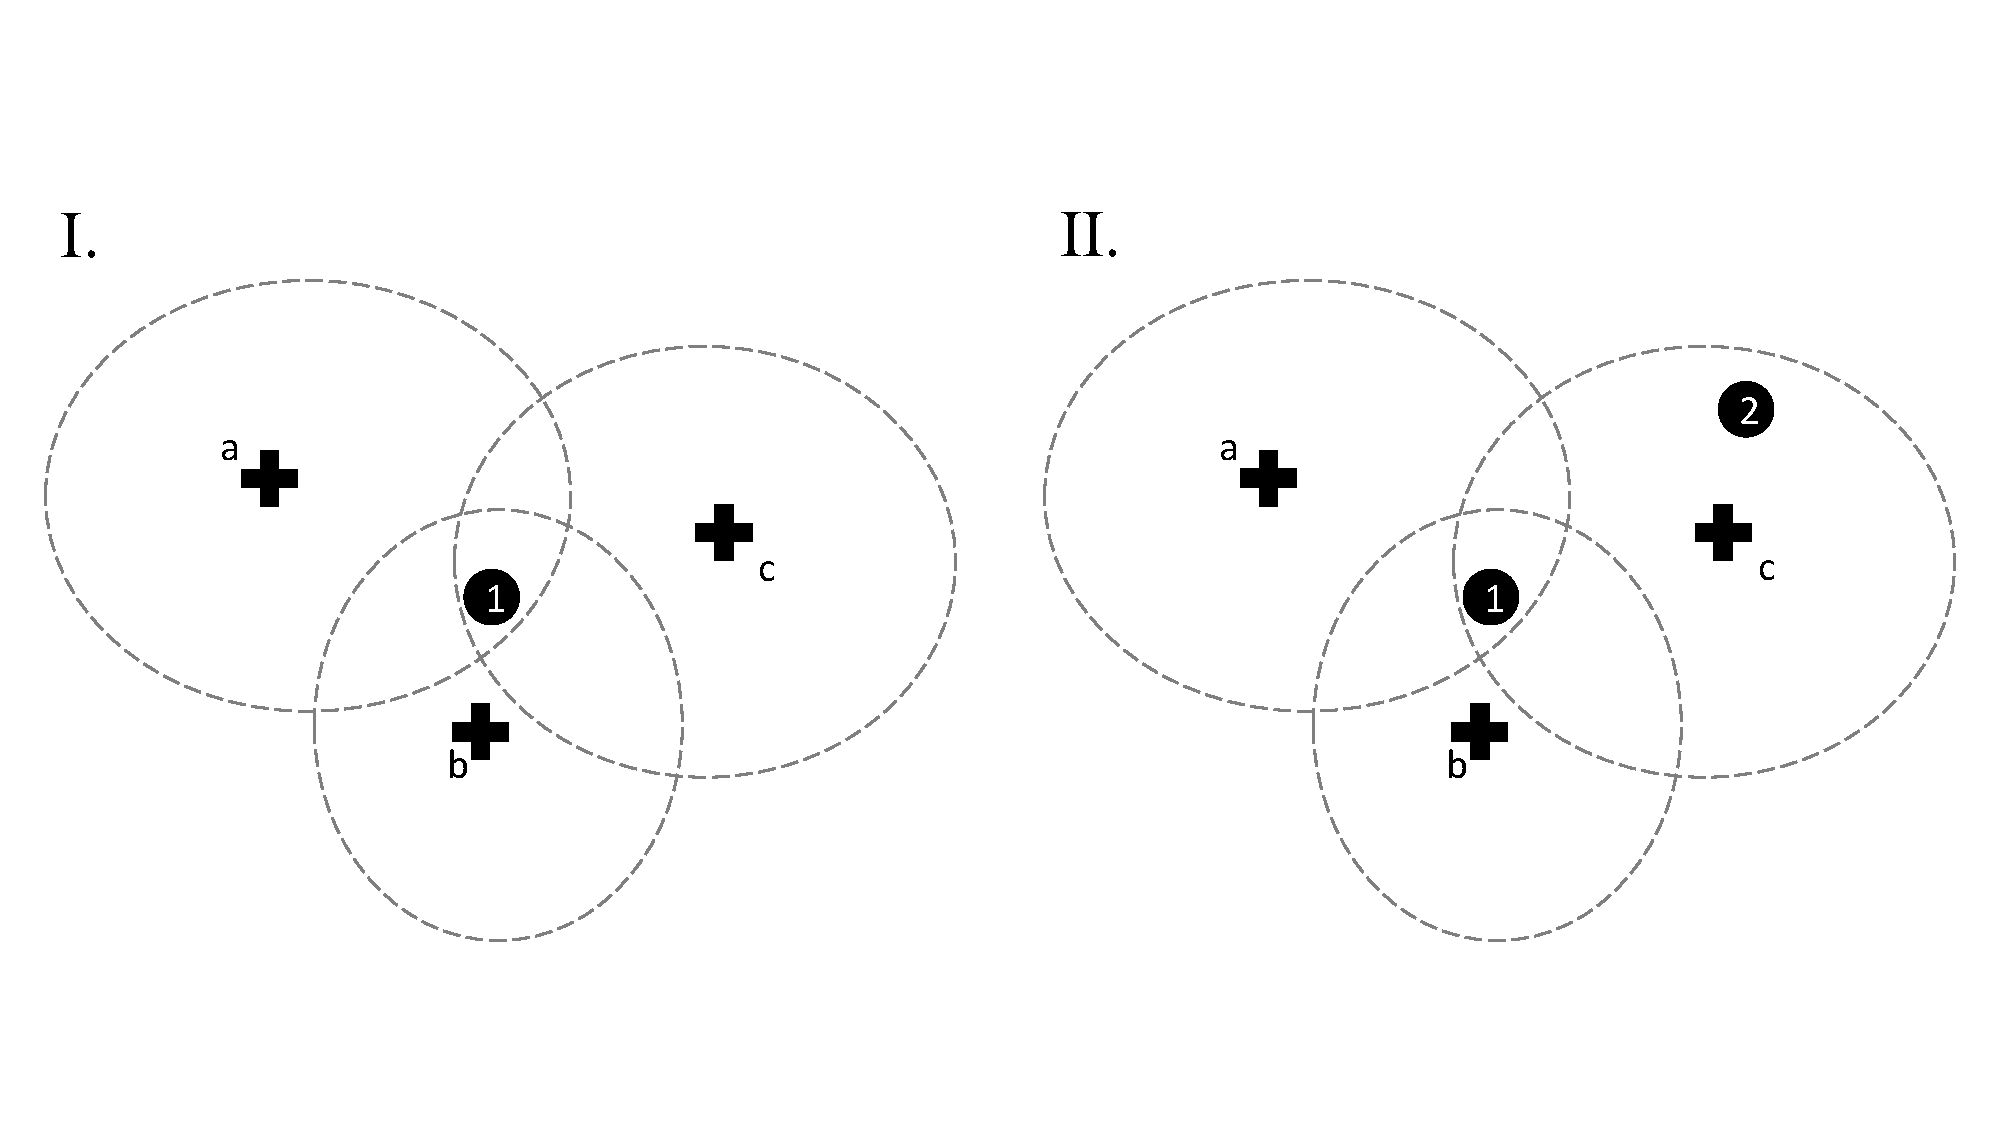
\includegraphics{fig1-Example1.pdf}
\caption{\label{fig:fig1-example-1}Example using binary impedance (the
dotted lines represent the impedance thresholds for each clinic)}
\end{figure}

A similar inflation effect is present on the supply side when the same
service point is included in the overlapping catchment areas of multiple
population centres. In this case, the same Local Clinic PPR is assumed
to be avalable to all those population centers, and therefore supply
becomes inflated in the second-stage calcuation of accessibility.
Continuing with the example, the 2SFCA algorithm assumes that the level
of service available at clinic \(c\) to population centers \(1\) and
\(2\) is both \(L_{1c}=L_{2c}=1/150\). In effect, the total level of
service available in the system at \(c\) for accessibility calculations
is actually \(2\) - twice the actual level of service at the clinic. In
the end, the accessibility for population center \(1\) is

\[
A_1 = 1/100 + 1/100 + 1/150 = 0.027
\] and population center \(2\) is \[
A_2 = 1/150 = 0.007
\] These accessibility results suggest that population center \(1\) has
a higher Local Population Center PPR than the Regional Average PPR of
0.020, while the accessibility of population center \(2\) falls below
the regional average. Of note, taking the population-weighted average of
the Local Population Center PPRs in the 2SFCA method returns the
Regional Average PPR. We will return to these results later.

\subsection{Demand and Supply Inflation in the
E2SFCA}\label{demand-and-supply-inflation-in-the-e2sfca}

The situation above becomes more vexing when using enhanced impedance
functions (i.e., non-binary). Such is the case of the enhanced 2SFCA
approach (E2SFCA), whereby the contribution of the population at \(i\)
to demand at service location \(j\) is: \[
D_{ij} = P_iW(d_{ij})
\]

An example of an impedance function is a stepwise function as follows
{[}12{]}: \[
W(d_{ij}) = \left\{
        \begin{array}{ll}
            1 & \quad d_{ij} \leq d_1 \\
            0.68 & \quad d_1 < d_{ij} \leq d_2 \\
            0.22 & \quad d_2 < d_{ij} \leq d_3 \\
            0 & \quad otherwise
        \end{array}
    \right.
\]

Let us revisit example (see Fig \ref{fig:fig2-example-2}, Panel I) now
using a stepwise impedance function. The population at \(1\) is still
within the catchment area of the three clinics (\(a\), \(b\), and
\(c\)), but now the impedance weights are \(W(d_{1a})=1\),
\(W(d_{1b})=0.68\), and \(W(d_{1c})=0.68\). If, as before, the
population at \(1\) is \(100\), the implied demand is inflated as
follows: \[
\sum_jD_{1j} = 100 + 68 + 68 = 236 > P_1 = 100
\]

Although inflation is lower in the case of the stepwise function
compared to the binary function, the same location \(i\) can still
potentially contribute multiple times its population value to different
service points \(j\), with similar consequences.

Turning to (see Fig \ref{fig:fig2-example-2}, Panel II), the implied
demand of population center \(2\), on the other hand, is: \[
\sum_jD_{2j} = 0 + 0 + 34 = 34 < P_2 = 50
\] and therefore demand has been \emph{deflated}.

This example demonstrates an internal contradiction in how FCA methods
operate: when multiple service centers are within the threshold travel
cost, they assume that some (maybe all) of the same persons crowd more
than one of those centers. On the other hand, when only one service
center is available, the assumption is that some individuals may
\emph{not} demand service, even when the center is within their
threshold travel cost. While this assumption may be acceptable for
discretionary services, it is suspect when it comes to essential
services such as primary health care.

\textbf{I am not sure about this next bit - the results in my excel
sheet are identical to those for the Binary solution. See email}

Continuing with this example, population center \(2\) (see Fig
\ref{fig:fig2-example-2}, Panel II) has an accessibility of 1 physician
per 118 people - higher than when the binary impedance function is used,
but still likely biased for two reasons: 1) demand from center \(1\) is
higher than the actual population; and 2) demand from center \(2\) is
lower than the actual population.

\begin{figure}
\centering
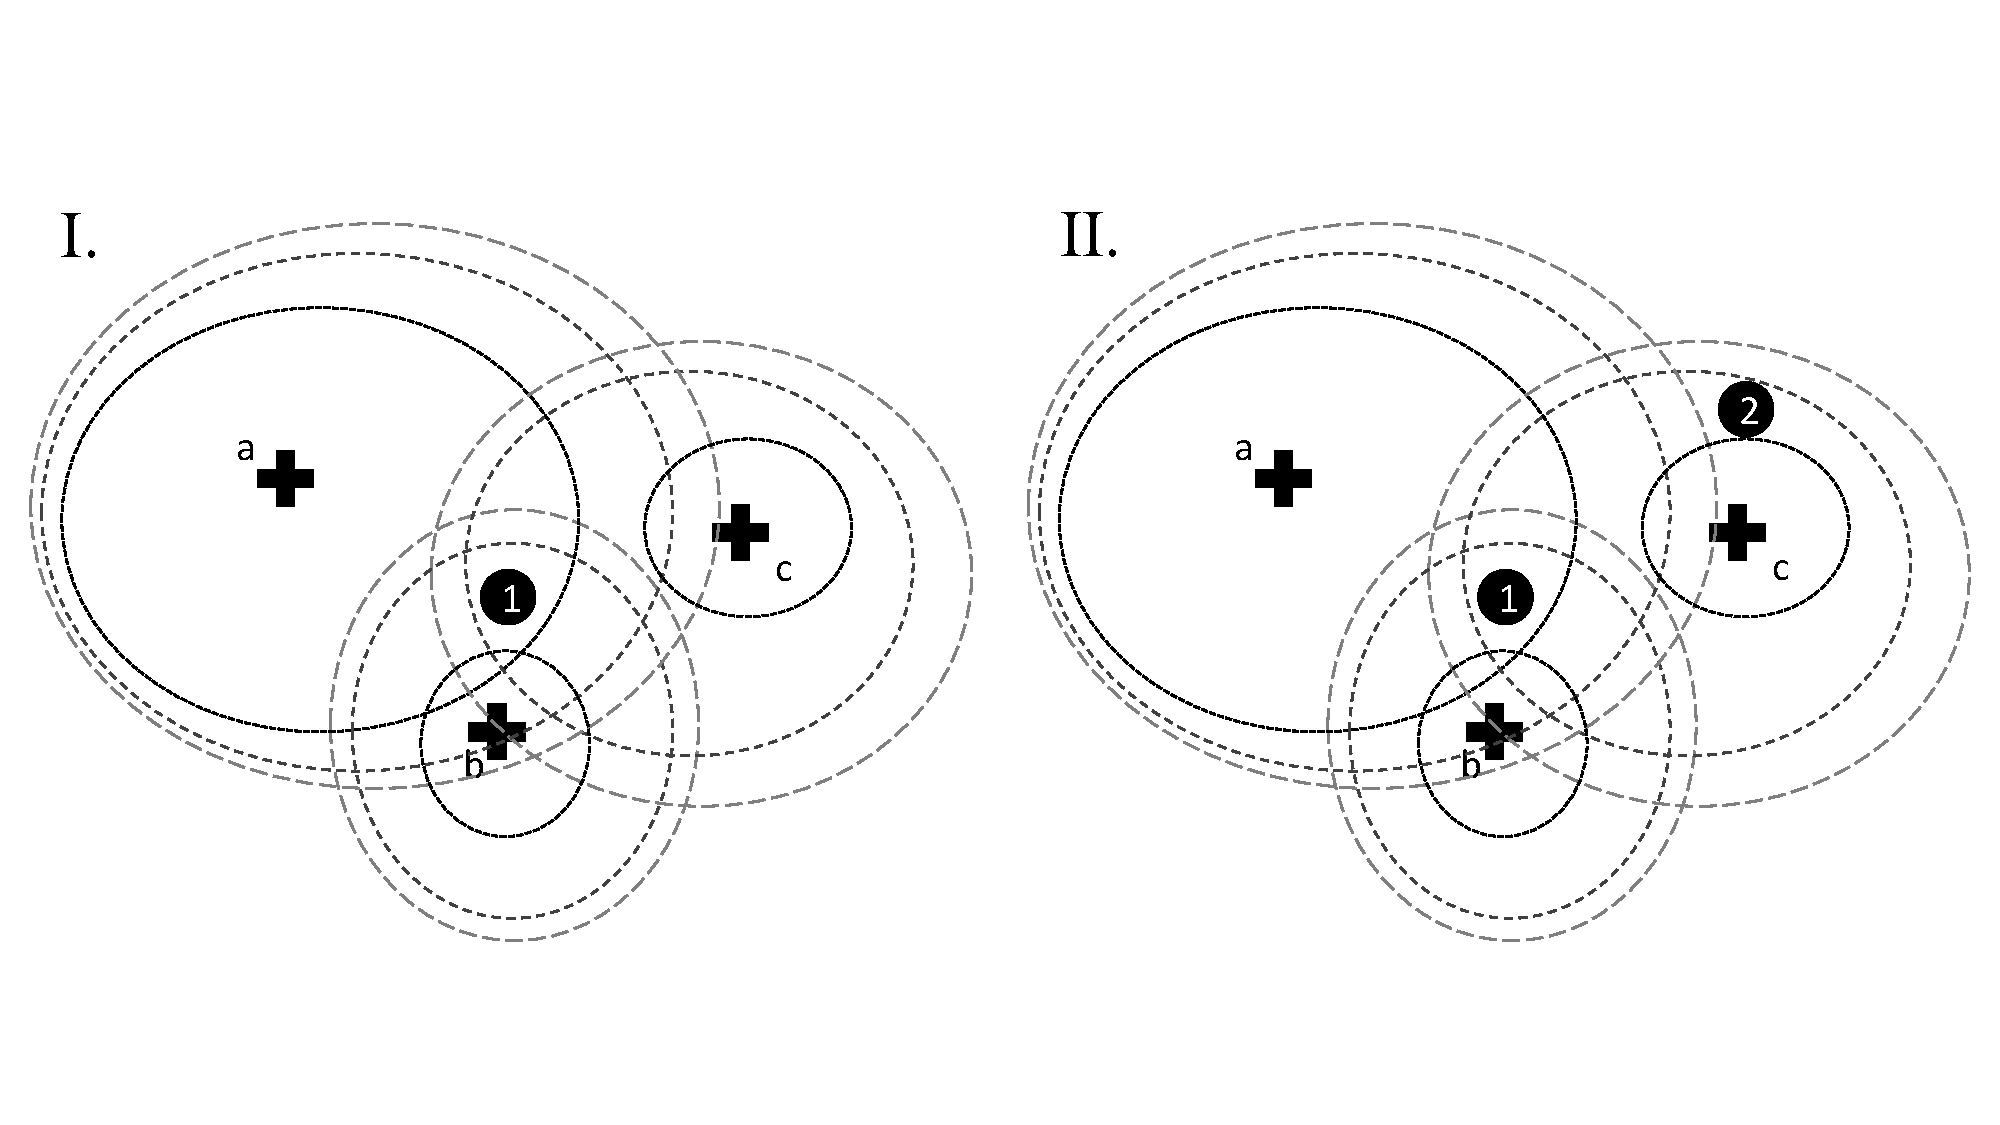
\includegraphics{fig2-Example2.pdf}
\caption{\label{fig:fig2-example-2}Congestion inflation and
accessibility deflation under stepwise impedance (each dotted line
represents a different impedance threshold)}
\end{figure}

\subsection{Demand and Supply Inflation in the
3SFCA}\label{demand-and-supply-inflation-in-the-3sfca}

Recognizing the potential for overestimated demand in the 2SFCA method,
Wan et al. {[}18{]} propose a 3-Step Floating Catchment Area method
(3SFCA) that aims at refining the estimates of level of demand and
accessibility by incorporating a \emph{selection weight}. This approach
operates by introducing an aditional step where selection weights are
calculated as follows: \[
G_{ij}=\frac{W(d_{ij})}{\sum_jW(d_{ij})}
\]

These selection weights are used to adjust the level of demand on the
second step of the algorithm in this fashion: \[
D^*_{ij} = G_{ij}P_iW_{ij} = G_{ij}D_{ij}
\]

The level of service at \(j\) is calculated in the second step as: \[
L_j=\frac{S_j}{\sum_iD^*_{ij}}
\]

Accessibility, in the final step, becomes: \[
A_i = \sum_jG_{ij}L_jW_{ij}
\]

But although it purports to fix overestimation in demand, the issue of
demand and supply inflation is not fully resolved by the 3SFCA method.
In this case, the selection weights are \(G_{1a} = 1/2.36\),
\(G_{1b} = 0.68/2.36\), \(G_{1c} = 0.68/2.36\) for location \(1\), and
\(G_{2a} = 0\), \(G_{2b} = 0\), \(G_{2c} = 0.68\) for location \(2\).
The adjusted levels of demand are then: \[
\begin{array}{l}
            D^*_{1a} = G_{1a}D_{1a} = (1/2.36)(100) = 42.37 \\
            D^*_{1b} = G_{1a}D_{1a} = (0.68/2.36)(68) = 19.59 \\
            D^*_{1c} = G_{1a}D_{1a} = (0.68/2.36)(68) = 19.59
\end{array}\quad \text{and}\quad
\begin{array}{ll}
            D^*_{2a} = G_{2a}D_{2a} = (0/0.68)(0) = 0 \\
            D^*_{2b} = G_{2b}D_{2b} = (0/0.68)(0) = 0 \\
            D^*_{2c} = G_{2b}D_{2c} = (0.68/0.68)(34) = 34
\end{array}
\]

It follows that the demand aggregated by population center is: \[
\sum_jD^*_{1j} = D^*_{1a} + D^*_{1b} + D^*_{1c} = 42.37 + 19.59 + 19.59 = 81.56 < P_1 = 100
\] for center \(1\), and: \[
\sum_jD^*_{2j} = D^*_{2a} + D^*_{2b} + D^*_{2c} = 0 + 0 + 34 = 34 < P_2 = 50
\] for center \(2\).

It appears from this example that the 3SFCA method has deflated demand
somewhat overzealously. This is perhaps not surprising, when we realize
that the 3SFCA method operates, essentially, by stacking the effects of
two related impedance functions (Delamater's {[}20{]} Modified 2SFCA
approach does the same but on the supply side). Recall that the
selection weights are calculated using the impedance weights
\(W(d_{ij})\). These selection weights then multiply the impedance when
computing the level of service (since \(D_{ij} = P_iW(d_{ij})\)). The
net effect is to make impedance steeper by a factor that depends on the
impedance {[}19{]}.

In addition to illustrating the demand/supply inflation (or deflation)
effect, the examples in this section also suggest that the magnitude and
even direction of the effect depend on the geography of the problem
(i.e., the locations of population centers and clinics), as well as the
kind of impedance function used. If the inflation effect were even
(i.e., all accessibility estimates are inflated/deflated at the same
rate) then a simple solution would be to apply a constant inflation
factor. Alas, it is more likely that the effect will not be even across
space (e.g., we can anticipate that demand will be more inflated in
denser parts of a region). For this reason, a more general approach to
offset the inflation of supply \emph{and} demand in a systematic way
seems to be called for. We discuss this next.

\subsection{A Method to Rectify Demand and Supply Levels to System-wide
Totals}\label{a-method-to-rectify-demand-and-supply-levels-to-system-wide-totals}

As the examples in the preceding subsection illustrate, FCA methods can
induce quite substantial inflation of supply and demand (and even, in
some cases, \emph{negative inflation}, or deflation). This, in turn, can
lead to artificially lower or higher estimates of accessibility, as the
case may be. In this section, we propose a simple and intuitive
adjustment to avoid the inflation artifacts inherent in current
implementations of FCA methods.

Refer again to Fig \ref{fig:fig1-example-1}. Demand inflation occurs
because the underlying assumption is that all the population within a
catchment area will be serviced by its corresponding service location.
More realistically, only a fraction of that population will demand
service at any given location if other service points are within reach
(i.e., inside its ``floated'' catchment area).

For instance, assuming (as the binary impedance function does), that
individuals at location \(1\) are indifferent between clinics \(a\),
\(b\), and \(c\), then it is reasonable to think that the population
will sort itself proportionally to the clinics - in this example, this
means that each third of the population will attend one of three
different clinics (importantly, this assumes that the service points
offer undifferentiated services). This suggests the following adjustment
to the way the level of demand is calculated. Given an impedance
function, a set of adjusted weights, say \(W^{i*}_{ij}\), are
precalculated by dividing the original impedance weights by the sum of
the weights for population center \(i\) over all service points \(j\):
\[
W_{ij}^{i} = \frac{W_{ij}}{\sum_j W_{ij}}
\]

Please notice that these weights are identical to the selection weights
of the 3SFCA method. A key property of the adjusted weights is the
following: \[
\sum_jW_{ij}^{i}=1
\]

This adjustment procedure has the effect that, when the level of demand
of \(i\) is summed over all service points \(j\), the aggregated level
of demand due to \(i\) is identical to its population: \[
\sum_j P_iW_{ij}^{i} = P_i
\]

On the supply side, inflation happens because the level of service
available at location \(j\) is assumed to be available to every
population center \(i\) within its catchment area. To adjust this,
another set of weights, say \(W^{j*}_{ij}\), is pre-calculated by
dividing the original impedance weights \(W_{ij}\) by the sum of the
weights for service point \(j\) over all population centers \(i\): \[
W_{ij}^{j} = \frac{W_{ij}}{\sum_i W_{ij}}
\]

Again, the resulting weights have the property that: \[
\sum_iW_{ij}^{j}=1
\]

As before, the result of this procedure is that, when the level of
service of \(j\) is aggregated by population centers, the total level of
service for that service point is preserved: \[
\sum_i L_jW_{ij}^{j} = L_j 
\]

Note that, since the weights add up to one, they can be interpreted as a
\emph{probability} or \emph{frequency} of contact, similar to the Huff
model of {[}19{]}.

In reference to Fig \ref{fig:fig1-example-1}, we can see that the
original (unadjusted) weights for population centre \(1\) are
\(W_{1a} = 1\), \(W_{1b} = 1\), and \(W_{1c} = 1\), whereas the weights
of population center \(2\) are \(W_{2a} = 0\), \(W_{2b} = 0\), and
\(W_{2c} = 1\).

On the demand side, the adjusted weights become for population center
\(1\), \(W^{i}_{1a} = 1/3\), \(W^{i}_{1b} = 1/3\), and
\(W^{i}_{1c} = 1/3\), and for population center \(2\)
\(W^{i}_{2a} = 0\), \(W^{i}_{2b} = 0\), and \(W^{i}_{2c} = 1\). Using
the adjusted weights, it can be seen that the level of demand due to
each population center equals its respective population: \[
\begin{array}{ll}
            \sum_j D_1j = 1/3P_1 + 1/3P_1 + 1/3P_1 = P_1\\
            \sum_j D_2j = 0+0+P_2 = P_2
        \end{array}
\]

Coming next to the supply side, the adjusted weights for service point
\(a\) are \(W^{j*}_{1a} = 1\) and \(W^{i*}_{2a} = 0\), for service point
\(b\) are \(W^{j*}_{1b} = 1\) and \(W^{i*}_{2b} = 0\), and for service
point \(c\) are \(W^{j*}_{1b} = 1/2\) and \(W^{i*}_{2b} = 1/2\). It can
be seen that the level of service is preserved across clinics, and
therefore across the system: \[
\begin{array}{ll}
            \sum_i L_{ia} = L_{1a} + 0 = L_a\\
            \sum_i L_{ib} = L_{1b} + 0 = L_b\\
            \sum_i L_{ic} = L_{1c}/2 + L_{2c}/2 = L_c
        \end{array}
\]

The method to adjust the weights used above is identical to a procedure
that will be familiar to readers acquainted with the literature in the
fields of spatial statistics and econometrics. The same adjustment is
widely used there under the names of row- and column-standardization of
a weights matrix {[}24,25{]}.

The proposed adjustment can be easily implemented. We will present next
the implementation using a compact matrix notation. Begin by defining
the following impedance matrix: \[
\mathbf{W} = \left(\begin{array}{ccc}
            W_{11} & \cdots & W_{1J}\\
            \vdots & \ddots & \vdots\\
            W_{N1} & \cdots & W_{NJ}\\
        \end{array}
        \right)
\] where \(W_{ij}\) is an impedance function evaluated at \(d_{ij}\).
Subindex \(i\) is for population centers (\(i=1,\dots,N\)) and subindex
\(j\) is for service points (\(j=1,\dots,J\)). Note that the matrix does
not need to be square. A row-standardized set of weights is obtained as
follows: \[
\mathbf{W}^{i} = \left(\begin{array}{ccc}
            \frac{W_{11}}{\sum_jD_{1j}} & \cdots & \frac{W_{1J}}{\sum_jD_{1j}}\\
            \vdots & \ddots & \vdots\\
            \frac{W_{N1}}{\sum_jD_{Nj}} & \cdots & \frac{W_{NJ}}{\sum_jD_{Nj}}\\
        \end{array}
        \right)
\]

Next, a column-standardized set of weights is calculated as: \[
\mathbf{W}^{j} = \left(\begin{array}{ccc}
            \frac{W_{11}}{\sum_iD_{1j}} & \cdots & \frac{W_{1J}}{\sum_iD_{1j}}\\
            \vdots & \ddots & \vdots\\
            \frac{W_{N1}}{\sum_iD_{Nj}} & \cdots & \frac{W_{NJ}}{\sum_iD_{Nj}}\\
        \end{array}
        \right)
\]

In the first example above (see Fig \ref{fig:fig1-example-1}), the
binary impedance matrix is: \[
\mathbf{W}_{binary} = \left(\begin{array}{ccc}
            1 & 1 & 1\\
            0 & 0 & 1\\
        \end{array}
        \right)
\]

The row-standardized weights that correspond to this matrix are: \[
\mathbf{W}^{i}_{binary} = \left(\begin{array}{ccc}
            1/3 & 1/3 & 1/3\\
            0 & 0 & 1\\
        \end{array}
        \right)
\] and the column-standardized weights are: \[
\mathbf{W}^{j}_{binary} = \left(\begin{array}{ccc}
            1 & 1 & 1/2\\
            0 & 0 & 1/2\\
        \end{array}
        \right)
\]

In the second example (see Fig \ref{fig:fig2-example-2}), the stepwise
impedance weights are: \[
\mathbf{W}_{stepwise} = \left(\begin{array}{ccc}
            1 & 0.68 & 0.68\\
            0 & 0 & 0.68\\
        \end{array}
        \right)
\]

The row-standardized weights in turn are (with some rounding): \[
\mathbf{W}^{i}_{stepwise} = \left(\begin{array}{ccc}
            0.424 & 0.288 & 0.288\\
            0 & 0 & 1\\
        \end{array}
        \right)
\] whereas the column-standardized weights are: \[
\mathbf{W}^{j}_{stepwise} = \left(\begin{array}{ccc}
            1 & 1 & 1/2\\
            0 & 0 & 1/2\\
        \end{array}
        \right)
\]

Once that the impedance weights have been adjusted, a vector of adjusted
level of demand \(\mathbf{D}^*\) can be obtained by multiplying the
\emph{transposed} impedance matrix by a vector of population values as
follows: \[
\mathbf{D}^* = [\mathbf{W}^{i}]^T\mathbf{P}
\] where the \(^T\) operator is for ``transpose'', and \(\mathbf{P}\)
is: \[
\mathbf{P} = \left(\begin{array}{c}
            P_1\\
            \vdots\\
            P_N\\
        \end{array}
        \right) 
\]

The level of demand for the service points in the binary impedance
function example is (in vector form): \[
\mathbf{D}^*_{binary}= \left( \begin{array}{cc}
1/3 & 0\\
1/3 & 0\\
1/3 & 1\end{array} \right)
\left( \begin{array}{c}
100\\
50\end{array} \right)=
\left( \begin{array}{c}
100/3\\
100/3\\
250/3
\end{array} \right)
\]

The level of demand for the service points in the stepwise impedance
function example is (in vector form): \[
\mathbf{D}^*_{sstepwise}= \left( \begin{array}{cc}
0.424 & 0\\
0.288 & 0\\
0.288 & 1\end{array} \right)
\left( \begin{array}{c}
100\\
50\end{array} \right)=
\left( \begin{array}{c}
42.4\\
28.8\\
78.8
\end{array} \right)
\]

As can be seen, the aggregated level of demand, after the adjustment,
equals (as desired) the total population of the region.

The levels of demand can then be introduced in the next stage of the
accessibility calculations by performing Hadamard division (\(\oslash\))
of the vector of supply by the vector of adjusted demand. This is the
first step of the 2SFCA (aggregating demand over catchment areas for
service points): \[
\mathbf{L}^* = \mathbf{S}\oslash\mathbf{D}^*
\]

Notice that levels of service are given in terms of units of supply per
units of demand, say physicians per person. This can be interpreted as
the provider-to-population ratio from the perspective of each service
point.

\textbf{Not correct} These values are consistent with the regional
provider-to-population ratio (RPRR), since: \[
RPPR = \frac{\sum_jS_j}{\sum_iD^*_i} = \frac{\sum_jS_j}{\sum_iP_i}
\]

The average of \(L^*\), on the other hand, can be interpreted as the
average clinic level of service, considering the spatial distribution of
supply and demand.

Since Hadamard division is an element-by-element operation, the adjusted
levels of service in the first example (using the binary impedance
function) are: \[
\mathbf{L}^*_{binary} = \left( \begin{array}{c}
1 \\
1 \\
1 \\
\end{array}\right)\oslash
\left( \begin{array}{c}
100/3\\
100/3\\
250/3
\end{array} \right)=
\left( \begin{array}{c}
3/100\\
3/100\\
3/250
\end{array} \right)=
\left( \begin{array}{c}
0.03\\
0.03\\
0.012
\end{array} \right)
\]

The levels of service in the second example, when using the stepwise
impedance function, are: \[
\mathbf{L}^*_{stepwise} = \left( \begin{array}{c}
1 \\
1 \\
1 \\
\end{array}\right)\oslash
\left( \begin{array}{c}
42.4\\
28.8\\
78.8
\end{array} \right)=
\left( \begin{array}{c}
0.024\\
0.035\\
0.013
\end{array} \right)
\]

Note that the values of level of service are consistent with the demand
and supply. As we saw above, the demand equals the population. Here, the
supply also equals the number of physicians in the region. Indeed, these
values are consistent with the Regional Average PPR of \(3/150\) or
\(0.02\) physicians per person. With this in mind, it is clear that
locations \(a\) and \(b\) offer better provider-to-population ratios
than the regional average, whereas location \(c\) offers a lower
provider-to-population than the regional average.

Accessibility, finally, is calculated as the matrix product of the
column-standardized weights and the adjusted level of service: \[
\mathbf{A}^*=\mathbf{W}^{j}\mathbf{L}^*
\] which, continuing with the example, gives the following for the
binary impedance function: \[
\mathbf{A}^*_{binary} = 
\left(\begin{array}{ccc}
            1 & 1 & 1/2\\
            0 & 0 & 1/2\\
        \end{array}
        \right)
\left( \begin{array}{c}
0.03\\
0.03\\
0.012
\end{array} \right) =
\left( \begin{array}{c}
0.03 + 0.03 + 0.006\\
0 + 0 + 0.006
\end{array} \right)=
\left( \begin{array}{c}
0.066\\
0.006
\end{array} \right)
\] and for the stepwise impedance function: \[
\mathbf{A}^*_{stepwise} = 
\left(\begin{array}{ccc}
            1 & 1 & 1/2\\
            0 & 0 & 1/2\\
        \end{array}
        \right)
\left( \begin{array}{c}
0.024\\
0.035\\
0.013
\end{array} \right) =
\left( \begin{array}{c}
0.024 + 0.035 + 0.0065\\
0 + 0 + 0.0065
\end{array} \right)=
\left( \begin{array}{c}
0.0655\\
0.0065
\end{array} \right)
\]

Notice that accessibility values are provider-to-population ratios as
perceived from the perspective of each population center, and therefore
are \emph{local} versions of the provider-to-population ratio.
Furthermore, the total accessibility in the system is identical to the
system-wide level of service, which in turn is consistent with the
supply and demand values of the system. To summarize, then, the
adjustment proposed succeeds at preserving the level of demand to the
total population, and the level of service to the total resources
available in the system. In this way, it provides a more intuitive
interpretation of accessibility.

\section{Empirical Example}\label{empirical-example}

In this and the following sections we present an empirical example to
illustrate the application of the methods. Based on the discussion
above, the adjusted 2SFCA employed in this research can be summarized
as:

\[
L_{j}=\sum_i\frac{S_j}{P_iW_{ij}^{i}}
\] with the incorporation of the row-standardized impedance weights
\(W_{ij}^i\) in the first step, and:

\[
A_i = \sum_j{L_jW_{ij}^{j}}
\] with the colum-standardized impedance weights \(W_{ij}^j\)
incorporated into the second step. The same approach is used to
re-weight the impedance function for the stepwise approach (i.e.,
E2SFCA). The case study is based on accessibility to family physicians
in the Hamilton CMA, in Ontario, Canada using data collected about the
distribution of the population and primary health care clinics (i.e.,
family physicians) in the region. Time use data from Canada's General
Social Survey was also used to inform the selection of thresholds for
the impedance functions. The data collection and preprocessing protocols
are described next.

\subsection{Family Physicians and Clinic
Locations}\label{family-physicians-and-clinic-locations}

In regards to the supply of clinics, the locations of family physicians
were obtained using the College of Physicians and Surgeons of Ontario
(CPSO) database for the Province of Ontario. We chose this organization
beacuse all physicians practicing in Ontario are required to register
with the CPSO, as set out in the Ontario Regulation 865/93: Registration
{[}26{]}.

Our search of CPSO's database was conducted attending to the following
criteria.

\begin{enumerate}
\def\labelenumi{\arabic{enumi})}
\item
  Only physicians who are registered as family physicians were selected
  (this excluded specialists such as pediatric physicians).
\item
  The spatial extent of the search was determined using forward
  sortation areas (FSAs), which are the first three initial characters
  of a postal code. Using a GIS, the regions of interest were selected
  by choosing FSAs within a 10 kilometer buffer distance from the
  Hamilton CMA boundary. This involved 72 different FSA regions. Each
  FSA region code was then searched in the CPSO database in addition to
  the family physician specification.
\end{enumerate}

The parameters of the search were deliberately conservative, and the
search identified a total of 2,224 family physicians practicing in the
region, of which, 864 are located in the Hamilton CMA. The resulting
dataset was manually verified by the third author to ensure that the
information was consistent and suitable for geocoding. Prior to
geocoding, locational information was organized in three columns,
containing street address, city name, and province name. After family
physicians were geocoded, locations were further examined. When family
physicians overlapped or were within a 50 meter distance of each other
we merged the records to identify 535 unique locations that we term
``clinics''. Many of these clinics are not in the Hamilton CMA proper,
but provide a buffer to minimize edge effects in the analysis. The
distribution of clinics and family physicians is shown in Fig
\ref{fig:fig3-clinic-map} for the Hamilton CMA.

\begin{figure}
\centering
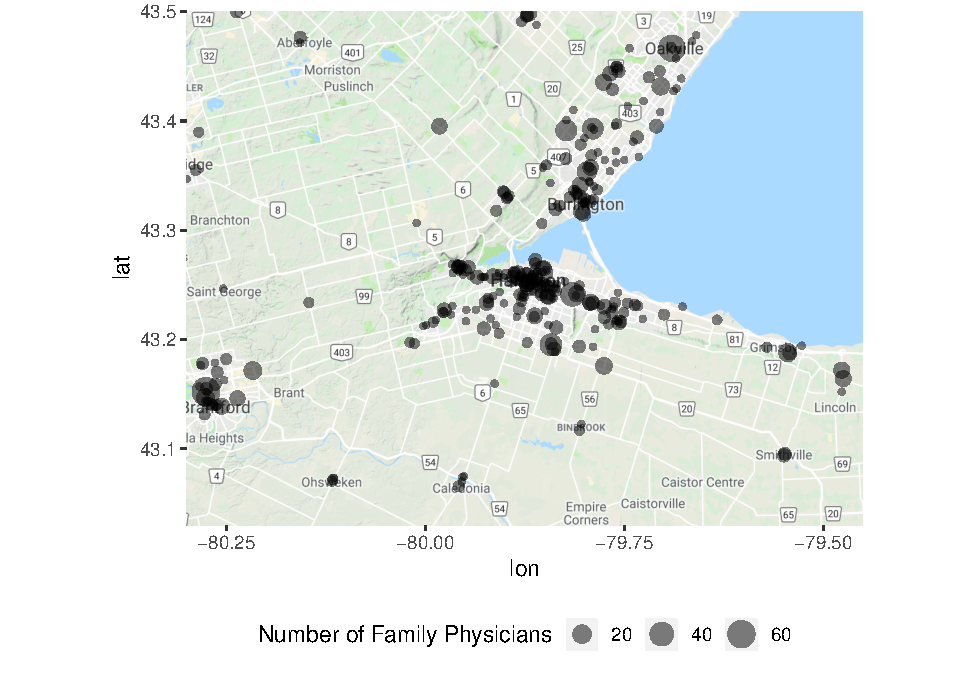
\includegraphics{Supply_and_Demand_Inflation_in_FCA_Methods_v2.0_files/figure-latex/fig3-clinic-map-1.pdf}
\caption{\label{fig:fig3-clinic-map}Location of clinics and family
physicians in the Hamilton CMA}
\end{figure}

\subsection{Population}\label{population}

Population information was obtained from the 2011 Canadian Census. To
maximize the spatial resolution, population data were acquired at the
Dissemination Area (DA) level of geography for all DAs within the
selected FSAs. As a result, this includes DAs not in the Hamilton CMA
proper, but that provide a buffer against edge effects. From this, the
region contains a population of 2,959,090, of which 720,725 are in the
Hamilton CMA. The distribution of population in the Hamilton CMA is
shown in Fig \ref{fig:fig4-population-map}.

\begin{figure}
\centering
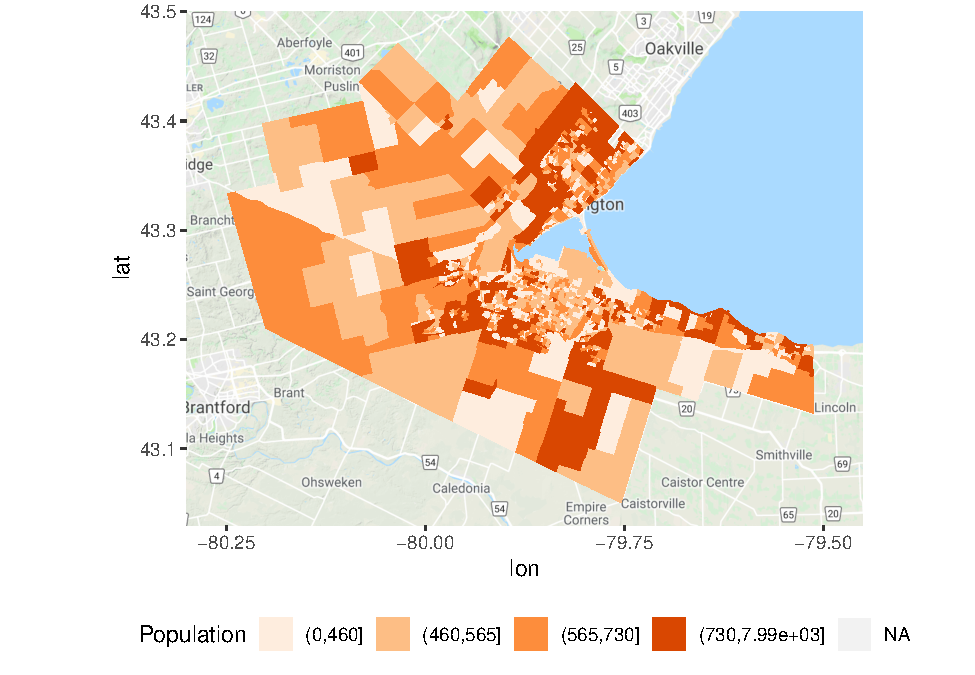
\includegraphics{Supply_and_Demand_Inflation_in_FCA_Methods_v2.0_files/figure-latex/fig4-population-map-1.pdf}
\caption{\label{fig:fig4-population-map}Population distribution in the
Hamilton CMA}
\end{figure}

\subsection{Travel Time Matrix}\label{travel-time-matrix}

Calculation of impedance weights requires that we evaluate an impedance
function at values of \(d_ij\), that is, the cost of travel between DA
\(i\) and clinic \(j\). In this research we used travel time as our cost
variable. To this end, we computed a matrix of travel times measured
over the road network. To calculate the travel time between population
centers and clinics we used the DA centroids and the geocoded locations
of clinics. Shortest paths on the network and subsequently travel times
were computed using a Geographic Information System.

\subsection{Impedance Functions}\label{impedance-functions}

For the experiments we used two different impedance functions,
corresponding to the 2SFCA and E2SFCA algorithms. We do not implement
the 3SFCA or the M2SFCA methods because, as noted above, they are
equivalent to using steeper impedances. For the 2SFCA apprach, impedance
is given by a binary function, whereas for E2SFCA it is given by a
stepwise function. The impedance functions require that we define cost
(i.e., travel time) thresholds to implement them. To select the
thresholds, we retrieved time use data from Canada's General Social
Survey Cycle 24 (see http://odesi2.scholarsportal.info/webview/).

From the time use files, we filtered all activity episodes corresponding
to respondents living in CMAs/CAs (metropolitan regions) in Ontario.
Next, we filtered all episodes taking place in a car (as driver) while
traveling for personal care activities for household adults (which
includes traveling to see a doctor) and traveling for shopping or
obtaining services (which includes traveling to go to health clinic or
doctor's office). It is worthwhile noting that travel by car accounts
for over 95\% of trips for the selected purposes in Ontario CMAs/CAs.

Once episodes were filtered by mode of travel and purpose of the trip,
their durations (in minutes) were examined by means of quantile
analysis, using episode weights to ensure representativeness of the
analysis. From the results, we learned that 50\% of all trips by car for
the aforementioned purposes are less than 15 minutes long, and we
selected this value as the threshold \(d_0\) for the binary function. In
other words, this part of the analysis assumes that any person who has
to travel longer than 15 minutes to reach a clinic is outside of its
catchment area. We deem this value appropriate for the scale, density,
and level of congestion of Hamilton CMA.

Quantile analysis of trip durations was used to calibrate a Gaussian
function with standard deviation set at 15 minutes, to match the value
selected for the binary impedance above. This produced the following
stepwise function, with any trips longer than 45 minutes assumed to be
outside of catchment: \[
W(d_{ij}) = \left\{
        \begin{array}{ll}
            0.946 & \quad d_{ij} \leq 5 \\
            0.801 & \quad 5 < d_{ij} \leq 10 \\
            0.607 & \quad 10 < d_{ij} \leq 15 \\
            0.411 & \quad 15 < d_{ij} \leq 20 \\
            0.135 & \quad 20 < d_{ij} \leq 30 \\
            0.011 & \quad 30 < d_{ij} \leq 45 \\
            0.00 & \quad 45 < d_{ij}
        \end{array}
    \right.
\]

Notice how the stepwise function has weights greater than 0.5 for
\(d_{ij} \leq 15 min\) and less than 0.5 for \(d_{ij} > 15 min\). This
means that it will count fewer people than the binary function when
\(d_{ij} \leq 15 min\), but more when \(d_{ij} > 15 min\).

\section{Results}\label{results}

We begin our discussion of the results by noting that with a total
population of the region of 2,959,090 and 2,224 family physicians, the
regional provider-to-population ratio is 0.752 family physicians per
1,000 people. This value is somewhat lower than the value of 1.16 for
Ontario reported by CIHI {[}27{]} and lower than the 1.20 estimated
based on the population and physician data for the Hamilton CMA, which
we attribute to our conservative search criteria of family physicians in
the rest of the region.

The level of demand is calculated for the 2SFCA and E2SFCA using both
the unadjusted and adjusted impedance matrices. Table
\ref{tab:table-descriptive-statistics} reports the total level of demand
calculated by each impedance matrix. As seen there, when no adjustment
is made, demand explodes to several times the actual population in the
region. However, when the impedance weights are standardized, demand is
now only slightly less than the total population for the region, since a
small proportion of the population turns out to be outside of catchment
areas. The total demand under binary impedance is lower due to the more
strict catchment area condition (i.e., less than 15 minutes), compared
to the stepwise function (i.e., less than 45 minutes), which in turn is
somewhat lower than the total demand in the regional
provider-to-population ratio, which does not impose catchment area
constraints within the region.

It is clear that the rectified demand leads to results that are
considerably more realistic. This is also seen when calculating the
provider-to-population ratios for each case (i.e., Family Physicians per
1,000 people). As seen in Fig \ref{fig:fig5-map-demand-inflation-binary}
and Fig \ref{fig:fig6-map-demand-inflation-stepwise}, demand inflation
is far from uniform. Inflation factors are also substantially higher
when the binary impedance function is used. Since this function lacks a
gradual distance-decay mechanism, it is more generous in terms of
counting population serviced.

\begin{table}[t]

\caption{\label{tab:table-descriptive-statistics}\label{tab:table-descriptive-statistics}Descriptive Statistics}
\centering
\begin{tabular}{llr}
\toprule
Case & Total Demand & Family Physicians per 1,000\\
\midrule
Binary & 143,655,060 & 0.015\\
Binary Adjusted & 2,857,595 & 0.778\\
Stepwise & 171,081,702 & 0.013\\
Stepwise Adjusted & 2,955,670 & 0.752\\
\bottomrule
\end{tabular}
\end{table}

\begin{figure}
\centering
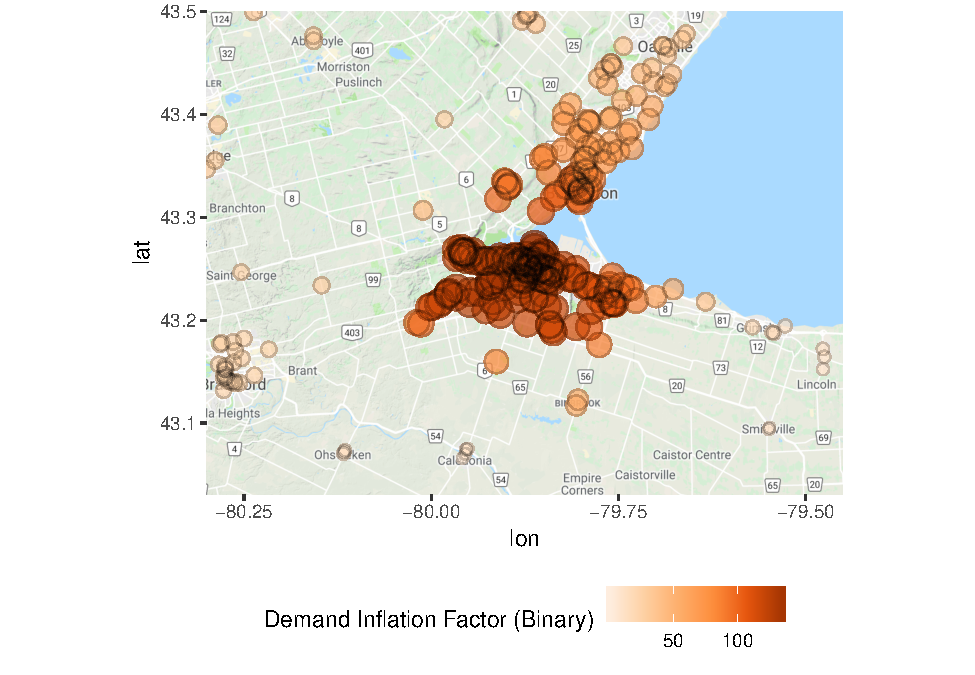
\includegraphics{Supply_and_Demand_Inflation_in_FCA_Methods_v2.0_files/figure-latex/fig5-map-demand-inflation-binary-1.pdf}
\caption{\label{fig:fig5-map-demand-inflation-binary}Demand inflation,
binary impedance function}
\end{figure}

\begin{figure}
\centering
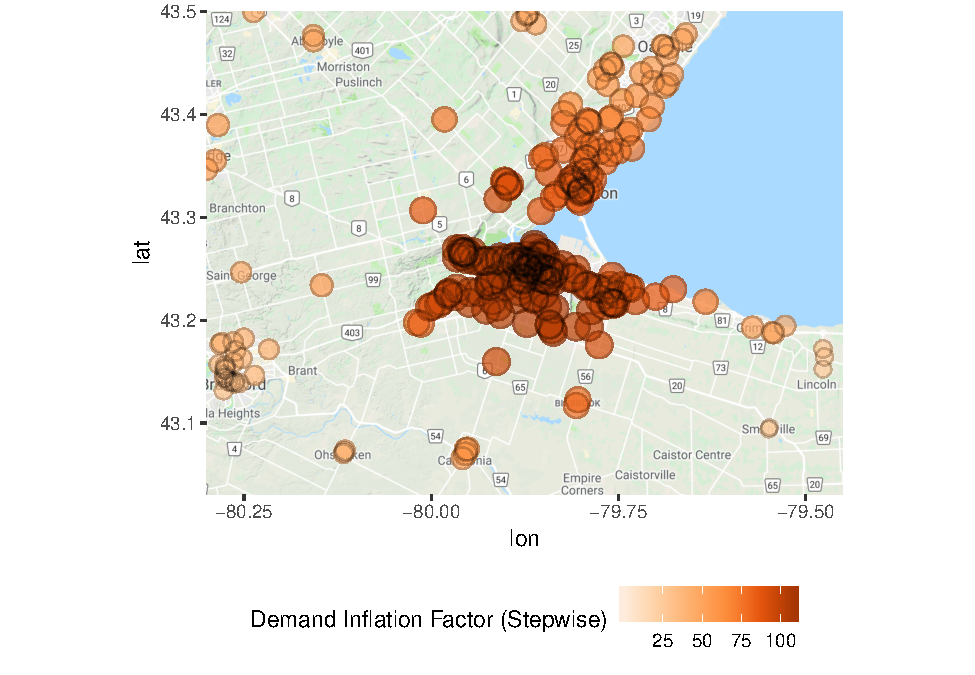
\includegraphics{Supply_and_Demand_Inflation_in_FCA_Methods_v2.0_files/figure-latex/fig6-map-demand-inflation-stepwise-1.pdf}
\caption{\label{fig:fig6-map-demand-inflation-stepwise}Demand inflation,
stepwise impedance function}
\end{figure}

The next step in the algorithm is to calculate the levels of service,
that is, the number of physicians (supply) by level of demand. Since in
the case of the adjusted impedance weights the demand is rectified to
the population, the level of service is likely going to be higher than
when the unrectified demand is used as in the conventional 2FSCA and
3SFCA implementations. Higher levels of service, however, do not
necessarily translate in the second step of the algorithm into higher
accessibility, since levels of service are also rectified so that total
supply is not exceeded.

Accessibility maps for the implementation of 2SFCA are shown in Fig
\ref{fig:fig7-map-accessibility-binary} and Fig
\ref{fig:fig8-map-accessibility-binary-adjusted}. The general patterns
observed in the figures are as expected, with higher accessibility in
denser, better connected parts of the region. Relatively high
accessibility in the north and west of the CMA is due to proximity to
other major population centers such as Oakville, Kitchener, and
Waterloo.

\begin{figure}
\centering
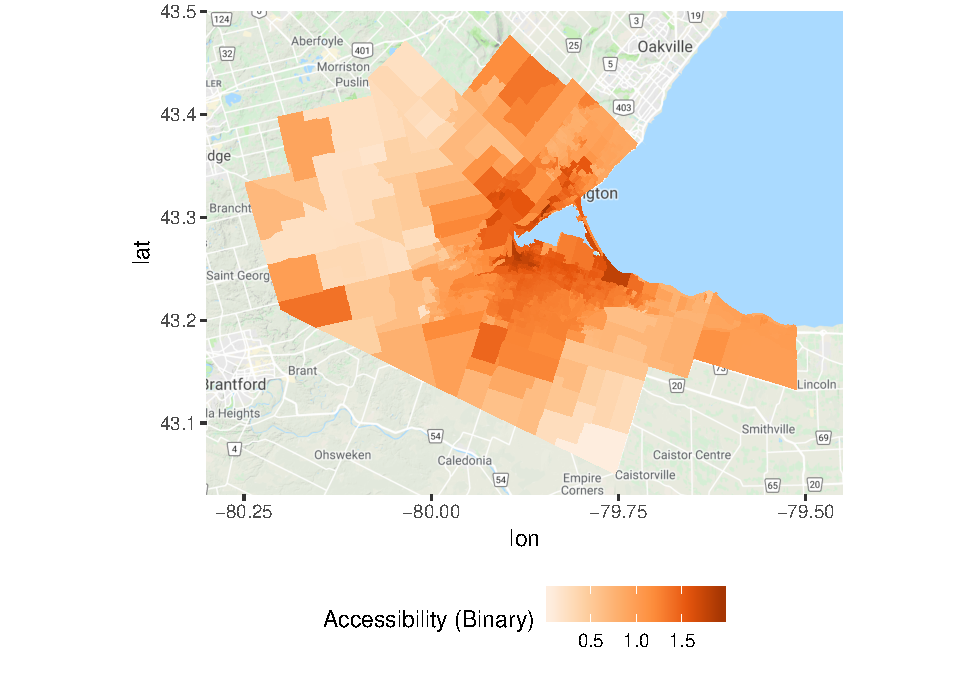
\includegraphics{Supply_and_Demand_Inflation_in_FCA_Methods_v2.0_files/figure-latex/fig7-map-accessibility-binary-1.pdf}
\caption{\label{fig:fig7-map-accessibility-binary}Accessibility, binary
impedance function}
\end{figure}

\begin{figure}
\centering
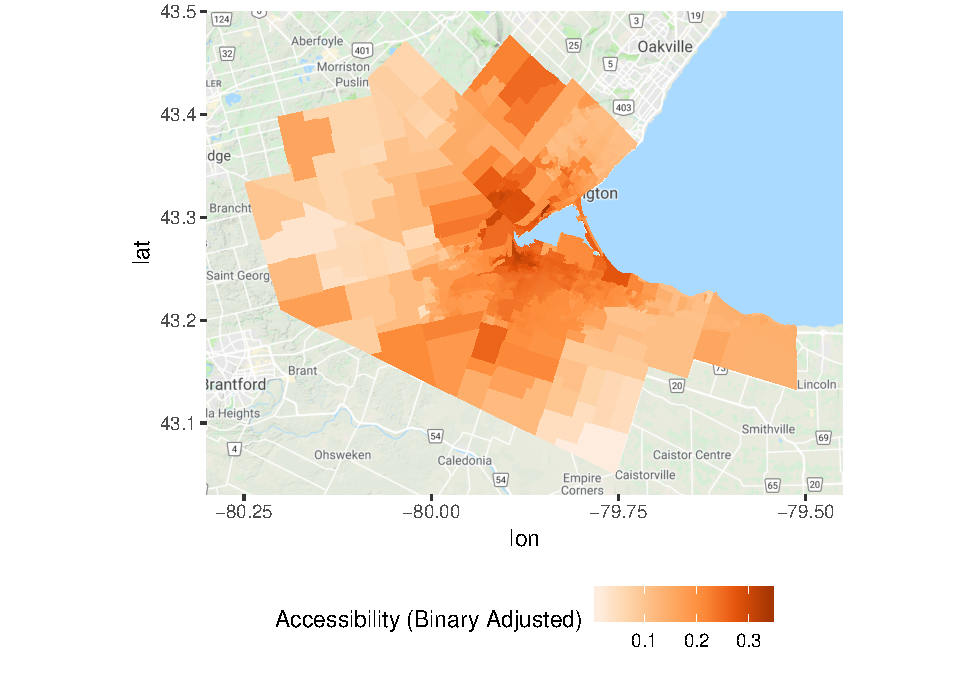
\includegraphics{Supply_and_Demand_Inflation_in_FCA_Methods_v2.0_files/figure-latex/fig8-map-accessibility-binary-adjusted-1.pdf}
\caption{\label{fig:fig8-map-accessibility-binary-adjusted}Accessibility,
adjusted binary impedance function}
\end{figure}

The results demonstrate how inflation of the supply (i.e., the level of
service) leads to much higher values of accessibility in the case of the
binary 2SFCA method. The procedure to rectify the population and level
of service, on the other hand, leads to accessibility output that is in
line with the regional system-wide provider-to-population ratio. This,
in turn, makes interpretation of the output more robust and intuitive.

How much has access been inflated in the original 2SFCA? Fig
\ref{fig:fig9-map-accessibility-binary-comparison} plots the ratio of
the binary and adjusted binary accessibility measures. Here it can be
seen that the unadjusted accessibility values are at least three times
greater than their adjusted counterparts within the study area. This
inflation, moreover, is not uniform across space, with inflation of the
binary accessibility values up to 8 times greater than those from the
adjusted model at the edges of the city where the 15-minute catchment
areas begin to overlap with neighboring municipalites.

\begin{figure}
\centering
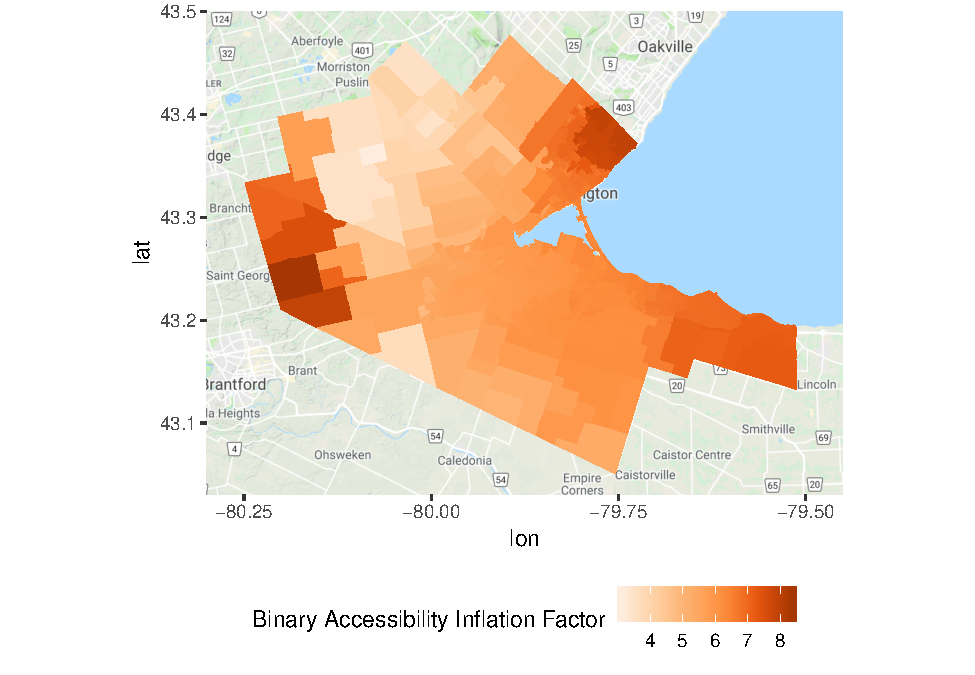
\includegraphics{Supply_and_Demand_Inflation_in_FCA_Methods_v2.0_files/figure-latex/fig9-map-accessibility-binary-comparison-1.pdf}
\caption{\label{fig:fig9-map-accessibility-binary-comparison}Accessibility
Inflation factor, binary impedance function}
\end{figure}

Why is this important? As noted by various authors {[}4,20{]}, in
traditional FCA methods, the sum of the population-weighted average of
accessibility across all population centers is equal to the regional
average provider-to-population ratio {[}20{]}. In the present case, the
weighted sum of accessibility in the unadjusted binary and stepwise
measures is 0.752. However, while this value is indeed identical to the
regional average provider-to-population ratio, it is problematic because
the share of the population correlates poorly with the pattern of
inflation observed (see Fig
\ref{fig:fig10-map-pop-share-inflation-comparison-binary}). The key
issue here is that accessibility is deflated by the share of the
population in a DA \(i\); however, the degree of inflation of demand and
supply depend not only of the population DA \(i\), but on the population
of every DA \(j\) with which DA \(i\) interacts via coincident catchment
areas. As a consequence, deflating accessibility using population shares
in previous FCA methods does not accurately offset demand and supply
inflation.

\begin{figure}
\centering
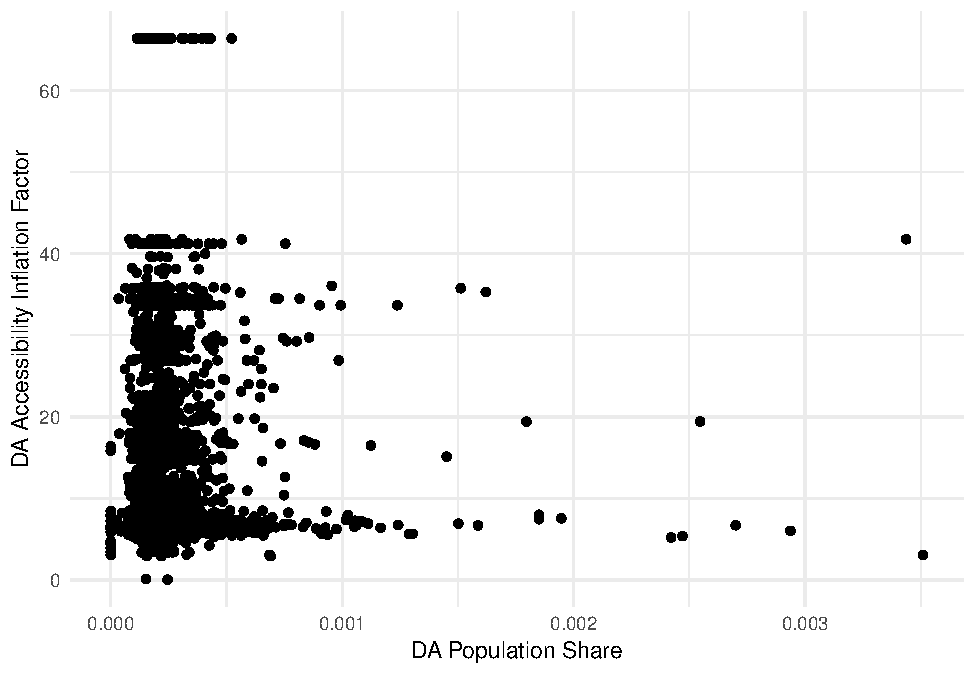
\includegraphics{Supply_and_Demand_Inflation_in_FCA_Methods_v2.0_files/figure-latex/fig10-map-pop-share-inflation-comparison-binary-1.pdf}
\caption{\label{fig:fig10-map-pop-share-inflation-comparison-binary}Population
share and inflation factors compared}
\end{figure}

Fig \ref{fig:fig11-map-accessibility-stepwise} and Fig
\ref{fig:fig12-map-accessibility-stepwise-adjusted} present the results
for the stepwise E2SFCA with and without the rectification. The results
are qualitatively similar to the 2FSCA, with the expected differences.
The inflation factor is even more substantial, given the larger
catchment areas used.

\begin{figure}
\centering
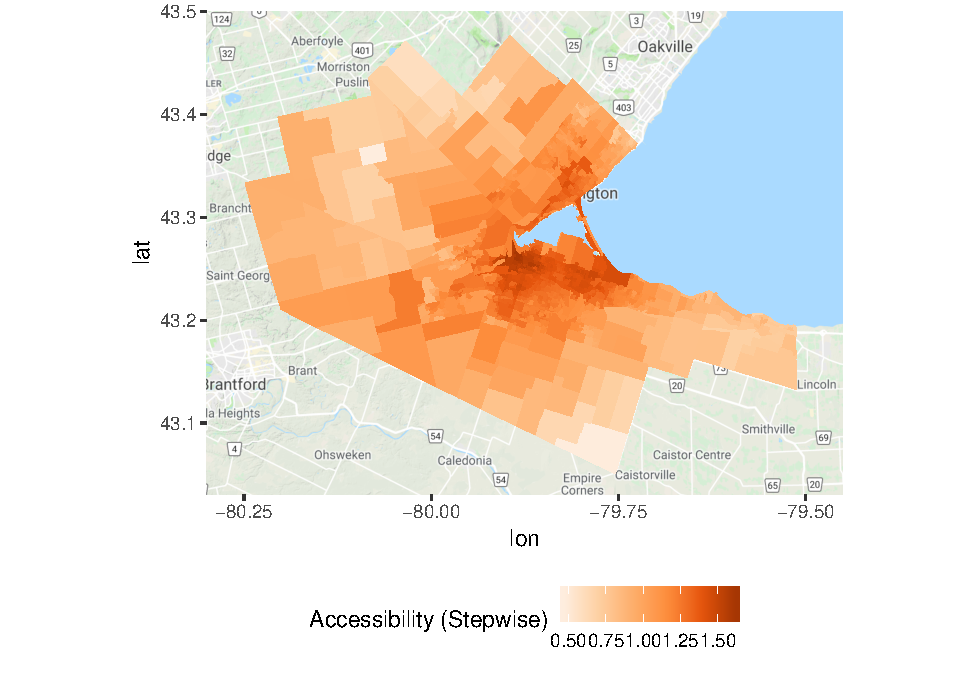
\includegraphics{Supply_and_Demand_Inflation_in_FCA_Methods_v2.0_files/figure-latex/fig11-map-accessibility-stepwise-1.pdf}
\caption{\label{fig:fig11-map-accessibility-stepwise}Accessibility,
stepwise impedance function}
\end{figure}

\begin{figure}
\centering
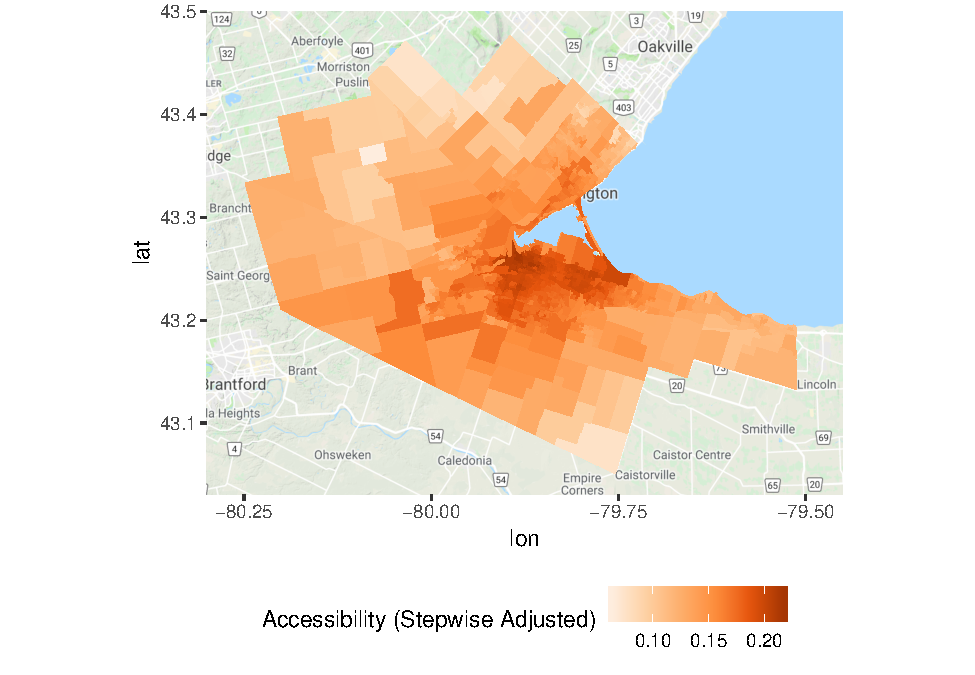
\includegraphics{Supply_and_Demand_Inflation_in_FCA_Methods_v2.0_files/figure-latex/fig12-map-accessibility-stepwise-adjusted-1.pdf}
\caption{\label{fig:fig12-map-accessibility-stepwise-adjusted}Accessibility,
adjusted stepwise impedance function}
\end{figure}

\begin{figure}
\centering
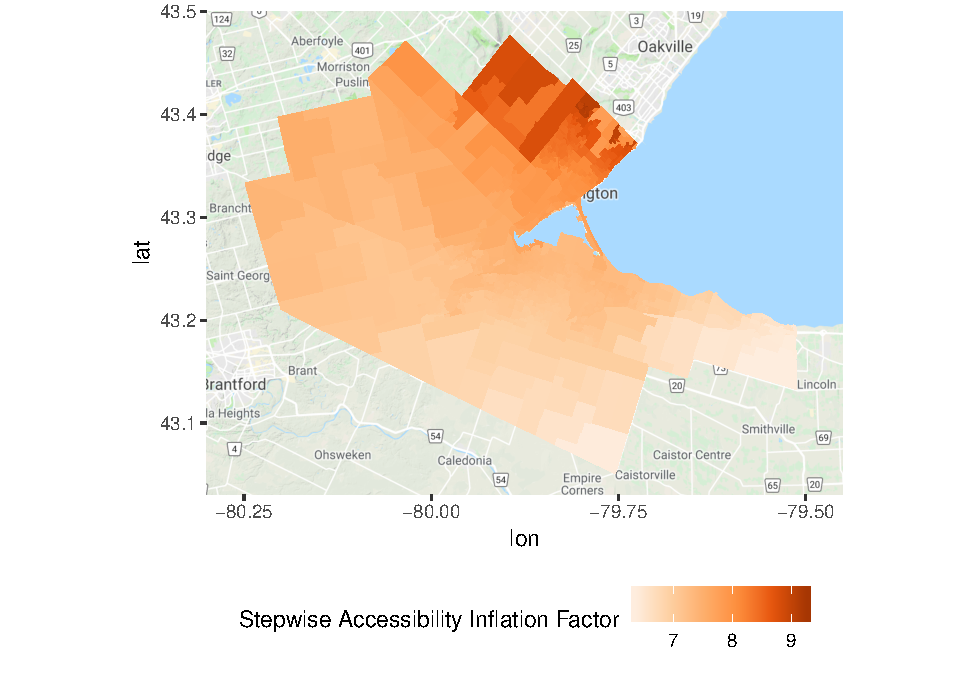
\includegraphics{Supply_and_Demand_Inflation_in_FCA_Methods_v2.0_files/figure-latex/fig13-map-accessibility-stepwise-comparison-1.pdf}
\caption{\label{fig:fig13-map-accessibility-stepwise-comparison}Accessibility
inflation factor, stepwise impedance function}
\end{figure}

\subsection{Disparity Analysis}\label{disparity-analysis}

Since neither supply or demand are inflated as in existing FCA methods,
it is possible to conduct accessibility disparity analysis in a very
intuitive way.

For instance, an analyst interested in equity analysis could allocate
the total level of service uniformly to every DA. In other words, the
total level of service (which equals the sum of accessibility over the
system) can be divided by the number of population centers in the
system. The resulting mean value, call it \(L_i^e\) then would be
assigned to the population centers as their ``equitable'' share of the
total level of service in the system. Next, the equitative distribution
of the level of service in each population center is substracted from
the estimated mean accessibility to arrive at a disparity index. When
the difference between these two quantities is positive, this would
indicate that a DA's accessibility exceeds its equitable share of level
of service. On the other hand, when the difference is negative, the DA's
accessibility is below its equitable share of the level of service.

This approach is reminiscent of the Spatial Access Ratio (SPAR) proposed
by Wan et al. {[}28{]}, which is calculated as the ratio between a
population center's accessibility and the mean accessibility across all
population centers. While Wan et al. {[}18{]} calculate SPAR based on
the results of their 3SFCA method, its use here with the adjusted demand
and supply parameters would enable more intuitive results. Nevertheless,
SPAR rescales the accessibility measures to reflect the percentage
difference in each population center's accessibility relative to the
mean and was designed to overcome the sensitivity of existing FCA
metrics to the impedance function. In contrast, the preservation of the
system-wide population and level of service in the adjusted approach
enables the disparity index to highlight the absolute difference in
accessible provider-to-population ratios across the population centers.

From this, the disparity maps for the binary and stepwise impedance
functions are shown in Fig \ref{fig:fig14-map-disparities-binary} and
Fig \ref{fig:fig15-map-disparities-stepwise}. These figures reveal the
spatial distribution in disparity, with levels of access that are lower
than the mean in more rural parts of the city (where travel times are
longer and the distribution of physicians is more spatially disperse)
compared to levels of access that are greater than the mean in the
higher-density and more connected urban center.

\begin{figure}
\centering
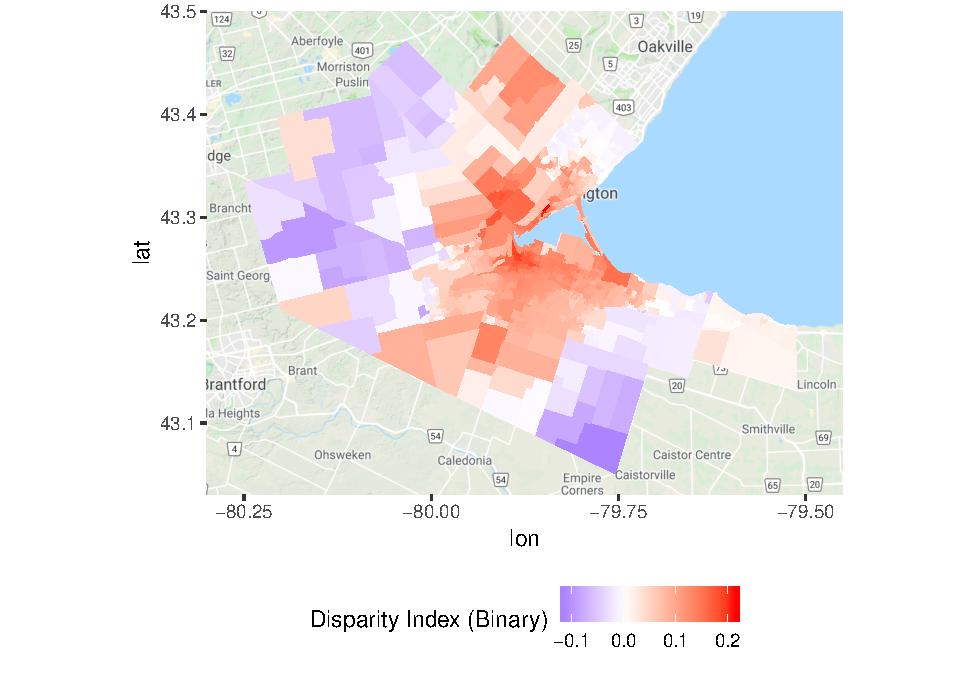
\includegraphics{Supply_and_Demand_Inflation_in_FCA_Methods_v2.0_files/figure-latex/fig14-map-disparities-binary-1.pdf}
\caption{\label{fig:fig14-map-disparities-binary}Accessibility
disparities, adjusted binary impedance function}
\end{figure}

\begin{figure}
\centering
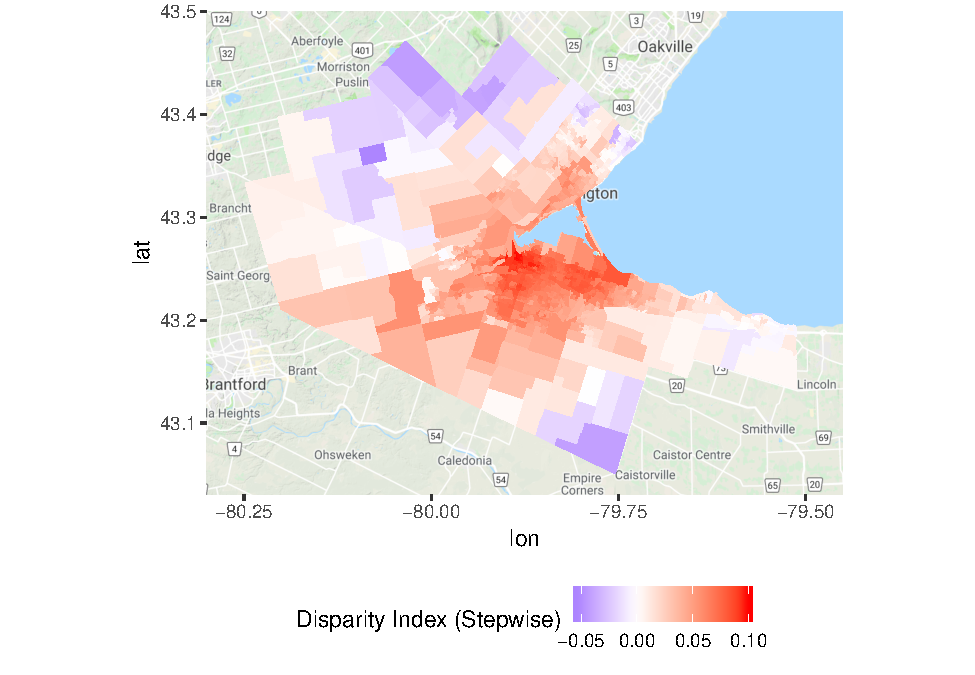
\includegraphics{Supply_and_Demand_Inflation_in_FCA_Methods_v2.0_files/figure-latex/fig15-map-disparities-stepwise-1.pdf}
\caption{\label{fig:fig15-map-disparities-stepwise}Accessibility
disparities, adjusted stepwise impedance function}
\end{figure}

\section{Conclusions}\label{conclusions}

Access to healthcare remains a critical issue in health geography. One
of the most popular approaches to estimating accessibility is the 2SFCA
method and its associated family of FCA models due to their
simplification of more complex gravity models and their interpretation
in terms of provider-to-population ratios. These intuitive properties
make FCA approaches particularly appealing for health policy. However,
the overestimation of demand in FCA approaches poses a serious challenge
to the interpretation of accessibility and the identification of spatial
disparities in access, with potentially deleterious consequences for
health policy.

Recognizing this, alternative approaches have been proposed that seek to
offset or minimize the demand overestimation problem. Nevertheless, the
present paper has shown that the inflation of demand is present in all
existing FCA methods. Moreover, we also show that in some cases, demand
is deflated, and detail the potential for inflation/deflation on the
supply side. To overcome these issues, we draw from spatial econometrics
to incorporate row-standardized impedance weights in the estimation of
an adjusted population demand parameter, and column-standardized
impedance weights to adjust the supply of physicians. These adjustments
ensure that the system-wide population and levels of service are
preserved in the estimation of accessibility, thereby rectifying the
inflation/deflation issue.

The case study application in Hamilton revealed the extent of inflation
in accessibility inherent in the unadjusted approaches compared to the
adjusted binary and stepwise FCA methods. Furthermore, the adjustments
result in local provider-to-population ratios which can be easily
understood relative to the system-wide equitable level of service
through the calculation of a disparity index. The applicability of these
values is particularly enhanced by the use of a travel survey to inform
the estimated impedance functions. Taken together, these innovations
provide estimates of spatial accessibility and disparity that are robust
to the regional distribution of supply and demand, as well as observed
travel behaviour. By extension, these properties mean that the adjusted
approach employed here can offer more rigorous recommendations for
health policy.

Our work is not without its limitations. For example, although we use a
travel survey to define their parameters, the use of binary and stepwise
impedance functions assumes a constant level of access within the
travel-time isochrones of a catchment area. While we employed these
functions for illustration purposes, the adjustment procedure outlined
here is also suitable for re-weighting continous impedance functions.
Second, our adjusted measures of supply and demand account for potential
interactions between all physicians and population in the system. This
is in contrast to Delamater's {[}20{]} M2SFCA, where some supply may not
be allocated due to the spatial configuration of opportunities relative
to population centers. Beyond overcoming the inflation issue inherent in
Delamater's modification, the assumption of full allocation in the
present case seems reasonable in the context of a single-payer
healthcare system with undifferentiated service. In essence, this
approach measures the potential for spatial interaction; whether or not
members of the population opt to actually use a given service is assumed
to be an outcome of the aspatial dimension of accessibility.

Nevertheless, the proposed adjustments overcome the inflation/deflation
issue inherent in previous FCA approaches. By incorporating these
methods into the estimation of accessibility to healthcare services,
future research can help to ensure that the FCA approach lives up to its
promise as an intuitive and policy-relevant method for investigating
access and disparity.

\section*{References}\label{references}
\addcontentsline{toc}{section}{References}

\hypertarget{refs}{}
\hypertarget{ref-Apparicio2017}{}
1. Apparicio P, Gelb J, Dube AS, Kingham S, Gauvin L, Robitaille E. The
approaches to measuring the potential spatial access to urban health
services revisited: Distance types and aggregation-error issues.
International Journal of Health Geographics. 2017;16.
doi:\href{https://doi.org/10.1186/s12942-017-0105-9}{10.1186/s12942-017-0105-9}

\hypertarget{ref-Joseph1982}{}
2. Joseph AE, Bantock PR. Measuring potential physical accessibility to
general practitioners in rural areas: A method and case study. Social
science \& medicine. Elsevier; 1982;16: 85--90.

\hypertarget{ref-Schuurman2010}{}
3. Schuurman N, Berube M, Crooks VA. Measuring potential spatial access
to primary health care physicians using a modified gravity model.
Canadian Geographer-Geographe Canadien. 2010;54: 29--45.
doi:\href{https://doi.org/10.1111/j.1541-0064.2009.00301.x}{10.1111/j.1541-0064.2009.00301.x}

\hypertarget{ref-Luo2003}{}
4. Luo W, Wang FH. Measures of spatial accessibility to health care in a
gis environment: Synthesis and a case study in the chicago region.
Environment and Planning B-Planning \& Design. 2003;30: 865--884.
Available:
\href{ISI:000187989500005\%0AC:/Papers/Environment\%20and\%20Planning\%20B/EPB\%20(2003)\%2030\%20(6)\%20865-885.pdf}{ISI:000187989500005
C:/Papers/Environment and Planning B/EPB (2003) 30 (6) 865-885.pdf}

\hypertarget{ref-Radke2000}{}
5. Radke J, Mu L. Spatial decomposition, modeling and mapping service
regions to predict access to social programs. Annals of Geographic
Information Sciences. 2000;6: 105--112.

\hypertarget{ref-Bauer2017}{}
6. Bauer J, Muller P, Maier W, Groneberg DA. Orthopedic workforce
planning in germany - an analysis of orthopedic accessibility. Plos One.
2017;12: 15.
doi:\href{https://doi.org/10.1371/journal.pone.0171747}{10.1371/journal.pone.0171747}

\hypertarget{ref-Kim2018}{}
7. Kim Y, Byon YJ, Yeo H. Enhancing healthcare accessibility
measurements using gis: A case study in seoul, korea. Plos One. 2018;13:
19.
doi:\href{https://doi.org/10.1371/journal.pone.0193013}{10.1371/journal.pone.0193013}

\hypertarget{ref-Fujita2017}{}
8. Fujita M, Sato Y, Nagashima K, Takahashi S, Hata A. Impact of
geographic accessibility on utilization of the annual health check-ups
by income level in japan: A multilevel analysis. Plos One. 2017;12: 14.
doi:\href{https://doi.org/10.1371/journal.pone.0177091}{10.1371/journal.pone.0177091}

\hypertarget{ref-Song2013}{}
9. Song PG, Zhu YJ, Mao X, Li Q, An L. Assessing spatial accessibility
to maternity units in shenzhen, china. Plos One. 2013;8: 7.
doi:\href{https://doi.org/10.1371/journal.pone.0070227}{10.1371/journal.pone.0070227}

\hypertarget{ref-McGrail2009}{}
10. McGrail MR, Humphreys JS. Measuring spatial accessibility to primary
care in rural areas: Improving the effectiveness of the two-step
floating catchment area method. Applied Geography. 2009;29: 533--541.
doi:\href{https://doi.org/10.1016/j.apgeog.2008.12.003}{10.1016/j.apgeog.2008.12.003}

\hypertarget{ref-Shah2016}{}
11. Shah TI, Bell S, Wilson K. Spatial accessibility to health care
services: Identifying under-serviced neighbourhoods in canadian urban
areas. Plos One. 2016;11.
doi:\href{https://doi.org/10.1371/journal.pone.0168208}{10.1371/journal.pone.0168208}

\hypertarget{ref-Luo2009}{}
12. Luo W, Qi Y. An enhanced two-step floating catchment area (e2sfca)
method for measuring spatial accessibility to primary care physicians.
Health \& Place. 2009;15: 1100--1107. Available:
\href{ISI:000270348400023\%0AC:/Papers/Health\%20and\%20Place/Health\%20and\%20Place\%20(2009)\%2015\%20(4)\%201100-1107.pdf}{ISI:000270348400023
C:/Papers/Health and Place/Health and Place (2009) 15 (4) 1100-1107.pdf}

\hypertarget{ref-Dai2010}{}
13. Dai D. Black residential segregation, disparities in spatial access
to health care facilities, and late-stage breast cancer diagnosis in
metropolitan detroit. Health \& place. Elsevier; 2010;16: 1038--1052.

\hypertarget{ref-Bauer2016}{}
14. Bauer J, Groneberg DA. Measuring spatial accessibility of health
care providers - introduction of a variable distance decay function
within the floating catchment area (fca) method. Plos One. 2016;11.
doi:\href{https://doi.org/10.1371/journal.pone.0159148}{10.1371/journal.pone.0159148}

\hypertarget{ref-Mao2013}{}
15. Mao L, Nekorchuk D. Measuring spatial accessibility to healthcare
for populations with multiple transportation modes. Health \& Place.
2013;24: 115--122.
doi:\href{https://doi.org/10.1016/j.healthplace.2013.08.008}{10.1016/j.healthplace.2013.08.008}

\hypertarget{ref-Ngui2011}{}
16. Ngui A, Apparicio P. Optimizing the two-step floating catchment area
method for measuring spatial accessibility to medical clinics in
montreal. Bmc Health Services Research. 2011;11. Available:
\url{http://www.biomedcentral.com/1472-6963/11/166}

\hypertarget{ref-Bell2013}{}
17. Bell S, Wilson K, Bissonnette L, Shah T. Access to primary health
care: Does neighborhood of residence matter? Annals of the Association
of American Geographers. Taylor \& Francis; 2013;103: 85--105.

\hypertarget{ref-Wan2012}{}
18. Wan N, Zou B, Sternberg T. A three-step floating catchment area
method for analyzing spatial access to health services. International
Journal of Geographical Information Science. 2012;26: 1073--1089.
doi:\href{https://doi.org/10.1080/13658816.2011.624987}{10.1080/13658816.2011.624987}

\hypertarget{ref-Luo2014}{}
19. Luo J. Integrating the huff model and floating catchment area
methods to analyze spatial access to healthcare services. Transactions
in GIS. Wiley Online Library; 2014;18: 436--448.

\hypertarget{ref-Delamater2013}{}
20. Delamater PL. Spatial accessibility in suboptimally configured
health care systems: A modified two-step floating catchment area
(m2sfca) metric. Health \& Place. 2013;24: 30--43.
doi:\href{https://doi.org/10.1016/j.healthplace.2013.07.012}{10.1016/j.healthplace.2013.07.012}

\hypertarget{ref-Taylor1971}{}
21. Taylor PJ. Distance transformation and distance decay functions.
Geographical Analysis. 1971;3: 221--238.
doi:\href{https://doi.org/doi:10.1111/j.1538-4632.1971.tb00364.x}{doi:10.1111/j.1538-4632.1971.tb00364.x}

\hypertarget{ref-Kwan1998}{}
22. Kwan MP. Space-time and integral measures of individual
accessibility: A comparative analysis using a point-based framework.
Geographical Analysis. 1998;30: 191--216. Available:
\href{ISI:000074579200001\%0AC:/Papers/Geographical\%20Analysis/Geographical\%20Analysis\%20(1998)\%2030\%20(3)\%20191-216.pdf}{ISI:000074579200001
C:/Papers/Geographical Analysis/Geographical Analysis (1998) 30 (3) 191-216.pdf}

\hypertarget{ref-Tobler1979}{}
23. Tobler WR. Smooth pycnophylactic interpolation for geographical
regions. Journal of the American Statistical Association. 1979;74:
519--530. Available:
\href{ISI:A1979HS22400001\%0AC:/Papers/Journal\%20of\%20the\%20American\%20Statistical\%20Association/Journal\%20of\%20the\%20American\%20Statistical\%20Association\%20(1979)\%2074\%20(367)\%20519-530.pdf}{ISI:A1979HS22400001
C:/Papers/Journal of the American Statistical Association/Journal of the American Statistical Association (1979) 74 (367) 519-530.pdf}

\hypertarget{ref-Anselin1988}{}
24. Anselin L. Spatial econometrics: Methods and models. Dordrecht:
Kluwer; 1988.

\hypertarget{ref-Griffith1988}{}
25. Griffith DA. Advanced spatial statistics: Special topics in the
exploration of quantitative spatial data series. Dordrecht: Kluwer;
1988.

\hypertarget{ref-Ontario1991}{}
26. 1991, Medicine Act, S.O. 1991, c. 30.

\hypertarget{ref-CIHI2018}{}
27. Health Information CI for. Number of physicians by
province/territory and specialty. Canadian Institute for Health
Information; 2018;

\hypertarget{ref-Wan2012SPAR}{}
28. Wan N, Zhan FB, Zou B, Chow E. A relative spatial access assessment
approach for analyzing potential spatial access to colorectal cancer
services in texas. Applied Geography. Elsevier; 2012;32: 291--299.

\nolinenumbers


\end{document}

